%%%%%%%%%%%%%%%%%%%%%%%%%%%%%%%%%%%%%%%%%%%%%%%%%%%%%%%%%%%%%%%%%%%%%%%%%%%%%%%%%%%%%%%%%
% Khóa luận tốt nghiệp/Tiểu luận 
% LaTeX Template
% Phiên bản 1.0 (tạo ra ngày 05/10/2022)
%
% Template này có thể được download tại:
% https://github.com/cpc1996/HUS-Dissertation-Template
%%%%%%%%%%%%%%%%%%%%%%%%%%%%%%%%%%%%%%%%%%%%%%%%%%%%%%%%%%%%%%%%%%%%%%%%%%%%%%%%%%%%%%%%%


%----------------------------------------------------------------------------------------
%	(KHÔNG CHỈNH SỬA PHẦN NÀY)
%
%	PHẦN 1: CÁC PACKAGE CƠ BẢN VÀ CÁC TÙY CHỈNH VĂN BẢN
%----------------------------------------------------------------------------------------

\documentclass[
12pt,
oneside,
english,
doublespacing,
nolistspacing,
liststotoc,
parskip,
headsepline,
chapterinoneline,
]{HUSdissertation}

% \usepackage[utf8]{inputenc} 
\usepackage[utf8]{vietnam} 
%\usepackage[T1]{fontenc}

\usepackage{mathptmx}
\usepackage{amsmath}
\usepackage{graphicx} 
\usepackage{array}
\allowdisplaybreaks

%https://www.overleaf.com/learn/latex/Biblatex_citation_styles
%\usepackage[backend=bibtex,style=authoryear,natbib=true]{biblatex}
\usepackage[backend=bibtex,style=numeric,citestyle=ieee,natbib=true]{biblatex}

\addbibresource{main.bib}

\usepackage[autostyle=true]{csquotes}


%----------------------------------------------------------------------------------------
%	PHẦN 2: CÁC PACKAGE BỔ TRỢ THÊM VÀO TRONG QUÁ TRÌNH BIÊN SOẠN
%----------------------------------------------------------------------------------------

\RequirePackage{setlst}		% Liệt kê/trích dẫn code

\usepackage{multirow}
\usepackage{subfigure}
\usepackage[fontsize=13pt]{scrextend}

%https://www.sascha-frank.com/latex-font-size.html
%https://tex.stackexchange.com/questions/103286/how-to-change-section-subsection-font-size
\usepackage{titlesec}

\titleformat{\section}
{\normalfont\fontsize{13}{13}\bfseries}{\thesection}{1em}{}

\titleformat{\subsection}
{\normalfont\fontsize{13}{13}\bfseries\itshape}{\thesubsection}{1em}{}

%https://tex.stackexchange.com/questions/351961/how-to-indent-code-in-beginverbatim
\usepackage{fancyvrb} 		% Fancy Verbatim
\fvset{tabsize=4,vspace=0pt,fontsize=\footnotesize}

\usepackage{longtable} 		% Bảng dài - Long table

\usepackage[figuresright]{rotating} % Bảng ngang - Sideways table
\usepackage{tabularx}

\usepackage{fontawesome5} 	% Các biểu tượng, ký hiệu đặc biệt

\usepackage{tikz} 			% Vẽ hình
\usetikzlibrary{calc}

\usepackage{indentfirst}	% Lùi đầu dòng ở đầu đoạn văn
\setlength{\parindent}{0.5cm}

%----------------------------------------------------------------------------------------
%	PHẦN 3: THÔNG TIN VỀ Khóa luận tốt nghiệp/Tiểu luận (THESIS INFORMATION)
%----------------------------------------------------------------------------------------

\author{Nhóm 2} 			
\thesistitle{Ứng dụng mạng nơ-ron tích chập (Convolutional Neural Network) trong nhận diện khẩu trang và cảm xúc} 

\supervisor {TS. Phạm Tiến Lâm} 
\supervisorr{Thầy Đặng Văn Báu} 

\field{Ngành Kỹ thuật Điện tử và Tin học} 				
\program{Chương trình đạo tạo chuẩn} 			
\doctype{Báo cáo kết thúc Học phần Học máy} 

\university{\href{http://hus.vnu.edu.vn}{Trường Đại học Khoa học Tự nhiên}}
\department{\href{http://hus.vnu.edu.vn/gioi-thieu/co-cau-to-chuc/khoa-truc-thuoc/khoa-vat-ly.html}{Khoa Vật lý}}

\AtBeginDocument{
	\hypersetup{pdftitle=\ttitle}
	\hypersetup{pdfauthor=\authorname}
}


\begin{document}

\lstset{style=codeC}	% Thiết lập ngôn ngữ C/C++ là ngôn ngữ mặc định cho phần liệt kê souce code của cả bài

\frontmatter 			% Sử dụng hệ thống đánh số La Mã (i, ii, iii, iv...) cho những trang trước phần mục lục

\pagestyle{plain} 


%----------------------------------------------------------------------------------------
%	(KHÔNG CHỈNH SỬA PHẦN NÀY)
%
%	PHẦN 4: TRANG TIÊU ĐỀ/TRANG BÌA (TITLE PAGE)
%----------------------------------------------------------------------------------------

% TRANG BÌA CHÍNH:
%----------------------------------------------------------------------------------------
%	(KHÔNG CHỈNH SỬA PHẦN NÀY)
%
%	Phần 6: TRANG TIÊU ĐỀ/TRANG BÌA (TITLE PAGE)
%----------------------------------------------------------------------------------------

% TRANG BÌA CHÍNH:
\begin{titlepage}
	\begin{tikzpicture}[overlay,remember picture]
		\draw [line width=3pt]
		($ (current page.north west) + (2.0cm,-2.0cm) $)
		rectangle
		($ (current page.south east) + (-1.5cm,1.8cm) $);
		\draw [line width=1pt]
		($ (current page.north west) + (2.15cm,-2.15cm) $)
		rectangle
		($ (current page.south east) + (-1.65cm,1.95cm) $); 
	\end{tikzpicture}
	\begin{center}
		
		\vspace{-.04\textheight}
		\noindent%\scshape
		\large \, \href{https://www.vnu.edu.vn/home/}{ĐẠI HỌC QUỐC GIA HÀ NỘI}\\
		\vspace{-0.25cm}{\large \MakeUppercase \univname}\\
		\vspace{-0.25cm}{\large \bfseries \MakeUppercase \deptname}\\[0.5cm]
		
\includegraphics{Logo/Logo_HUS_notext_nocolor}
		
		\vspace{1.0cm}
		
		{\large \MakeUppercase \authorname}
		
		\vspace{2.5cm}
		
		{\Large \bfseries \MakeUppercase\ttitle\par}
		
		\vspace{2.5cm}
		
		{\normalsize \docname\\ \fieldname\\ (\progname)\\}
		
		\vfill
		
		\textbf{Hà Nội - \the\year{}}
	\end{center}
\end{titlepage}



% TRANG BÌA PHỤ:
%----------------------------------------------------------------------------------------
%	(KHÔNG CHỈNH SỬA PHẦN NÀY)
%
%	Phần 6: TRANG TIÊU ĐỀ/TRANG BÌA (TITLE PAGE)
%----------------------------------------------------------------------------------------

% TRANG BÌA PHỤ:
\begin{titlepage}
	\begin{tikzpicture}[overlay,remember picture]
		\draw [line width=3pt]
		($ (current page.north west) + (2.0cm,-2.0cm) $)
		rectangle
		($ (current page.south east) + (-1.5cm,1.8cm) $);
		\draw [line width=1pt]
		($ (current page.north west) + (2.15cm,-2.15cm) $)
		rectangle
		($ (current page.south east) + (-1.65cm,1.95cm) $); 
	\end{tikzpicture}
	\begin{center}
		
		\vspace{-.04\textheight}
		\noindent%\scshape
		\large \, \href{https://www.vnu.edu.vn/home/}{ĐẠI HỌC QUỐC GIA HÀ NỘI}\\
		\vspace{-0.25cm}{\large \MakeUppercase \univname}\\
		\vspace{-0.25cm}{\large \bfseries \MakeUppercase \deptname}\\[0.5cm]
		
\includegraphics{Logo/Logo_HUS_notext}
		
		\vspace{1.0cm}
		
		{\large \MakeUppercase \authorname}
		
		\vspace{2.5cm}
		
		{\Large \bfseries \MakeUppercase\ttitle\par}
		
		\vspace{2.5cm}
		
		{\normalsize \docname\\ \fieldname\\ (\progname)\\}
		
		\vspace{2.5cm}
		
		\begin{minipage}[t]{0.49\textwidth}
			\begin{flushright} \large \bfseries
				Giảng viên hướng dẫn:\;
			\end{flushright}
		\end{minipage}
		\begin{minipage}[t]{0.5\textwidth}
			\begin{flushleft} \large \bfseries
				\supname\\
				\supnamee
			\end{flushleft}
		\end{minipage}
		
		\vfill
		
		\textbf{Hà Nội - \the\year{}}
	\end{center}
\end{titlepage}



%----------------------------------------------------------------------------------------
%	PHẦN 6: LỜI CẢM ƠN (ACKNOWLEDGEMENTS)
%----------------------------------------------------------------------------------------

\begin{acknowledgements}
	\addchaptertocentry{\acknowledgementname}
	\thispagestyle{empty}
	
	Trên thực tế không có sự thành công nào mà không gắn liền với những sự giúp đỡ dù ít hay nhiều, dù trực tiếp hay gián tiếp từ những người xung quanh. Trong suốt quá trình học tập và làm việc tại giảng đường tới nay, nhóm 2 đã nhận được nhiều sự quan tâm, giúp đỡ từ các thầy cô, gia đình và bạn bè. Nhóm 2 xin gửi lời cảm ơn chân thành nhất đến \textbf{TS. Phạm Tiến Lâm} và \textbf{Thầy Đặng Văn Báu} đã tận tâm hướng dẫn nhóm qua những buổi thảo luận, thực hành về môn học. Thầy đã giúp nhóm tích lũy thêm nhiều kiến thức, kĩ năng để có cái nhìn toàn diện ,sâu sắc và tính thiết thực mà môn học mang đến.
	
	Kiến thức là vô hạn mà sự tiếp thu tri thức của mỗi người là khác nhau và còn tồn tại những hạn chế nhất định. Do đó, trong quá trình hoàn thành bài báo cáo này, chắc chắn không tránh khỏi những thiếu sót. Nhóm 2 rất mong nhận được những ý kiến đóng góp quý báu từ thầy để bài báo cáo của nhóm được hoàn thiện hơn.
	
	Nhóm 2 xin kính chúc thầy sức khỏe và thành công trên sự nghiệp giảng dạy.
	
	\textbf{Nhóm 2 xin chân thành cảm ơn!}
	
	\begin{flushright}
		
		Trần Duy Nghĩa - 20002146\\
		Nguyễn Đình Quang - 20002155\\
		Hoàng Minh Quân - 20002156\\
		Phạm Xuân Tài - 20002161\\
		Nguyễn Thu Hà - 20002121\\
		
	\end{flushright}
\end{acknowledgements}


%----------------------------------------------------------------------------------------
%	(KHÔNG CHỈNH SỬA PHẦN NÀY)
%
%	PHẦN 7: MỤC LỤC (LIST OF CONTENTS/FIGURES/TABLES PAGES)
%----------------------------------------------------------------------------------------

\begin{spacing}{1.15}
	\tableofcontents 	% In ra mục lục chính
\end{spacing}

\begin{spacing}{1.15}
	\listoffigures 		% In ra danh sách hình vẽ
\end{spacing}

%\begin{spacing}{1.15}
	%\listoftables		% In ra danh sách bảng
%\end{spacing}


%----------------------------------------------------------------------------------------
%	PHẦN 8: DANH SÁCH TÊN VIẾT TẮT (ABBREVIATIONS)
%----------------------------------------------------------------------------------------

\begin{abbreviations}{ll} % Thêm danh sách tên viết tắt (dưới dạng một bảng có 2 cột)

\textbf{CNN} & \textbf{C}onvolutional \textbf{N}eural \textbf{N}etwork\\
\textbf{I/O} & \textbf{I}nput \textbf{O}utput \\
\textbf{ROM} & \textbf{R}ead \textbf{O}nly \textbf{M}emory\\
\textbf{RAM} & \textbf{R}andom \textbf{A}ccess \textbf{M}emory\\
\textbf{CPU} & \textbf{C}entral \textbf{P}rocessing \textbf{U}nit\\


\end{abbreviations}


%----------------------------------------------------------------------------------------
%	PHẦN 9: NỘI DUNG/CÁC CHƯƠNG Khóa luận tốt nghiệp/Tiểu luận (THESIS CONTENT - CHAPTERS)
%----------------------------------------------------------------------------------------

\mainmatter % Bắt đầu đánh số trang (1,2,3...)

\pagestyle{plain}

% Hãy thêm những chương (chapter) của khóa luận/tiểu luận vào thư mục Chapters
% Hãy bỏ chú thích những dòng nếu bạn đã bổ sung những chương vào

\chapter*{LỜI MỞ ĐẦU}
\addcontentsline{toc}{chapter}{MỞ ĐẦU}

\label{Chapter0} 

Machine Learning đã và đang đóng góp một vai trò quan trọng trong tất cả các lĩnh vực trên toàn thế giới, mỗi năm có hàng ngàn báo cáo khoa học về đề tài này. Các công ty công nghệ hàng đầu như Google, Facebook, Amazon và Microsoft đang đầu tư mạnh mẽ vào học máy để phát triển các sản phẩm và dịch vụ mới. Ngoài ra, học máy cũng đang được sử dụng rộng rãi trong các lĩnh vực như y tế, tài chính, sản xuất và nhiều lĩnh vực khác để cải thiện hiệu suất và tối ưu hóa quy trình.

Những năm gần đây, khi mà khả năng tính toán của các máy tính được nâng lên một tầm cao mới và lượng dữ liệu khổng lồ được thu thập, Machine Learning đã tiến thêm một bước dài và Deep Learning ra đời. Deep Learning đã giúp máy tính thực thi những công việc phức tạp hơn như: phân loại cả ngàn vật thể trong các bức ảnh, tạo chú thích cho ảnh, bắt chước giọng nói và chữ viết của con người, giao tiếp với con người...

Theo số liệu thống kê của Google cho đến thời điểm hiện tại, về tình hình dịch bệnh trên toàn thế giới. 

Trên toàn thế giới có hơn 649.799.405 triệu ca nhiễm, đã bình phục 626.994.443 và tổng số ca tử vong đã lên đến 6.646.043 triệu ca. Con số ca nhiễm và số tử vong vẫn không có dấu hiệu ngừng tăng.

Riêng đối với Việt Nam tính ngày 01/06/2023 đã có tổng số ca nhiễm là 11.602.738 triệu ca, trong đó đã có 10.635.065 triệu ca đã bình phục và 43.203 ca đã tử vong. Mỗi ngày vẫn còn khoảng 240 ca nhiễm covid .  Đó là một con số không hề nhỏ và đáng bảo động.

Ở nước ta, từ đầu năm 2020 đến nay đã sảy ra nhiều ca tử vong đáng tiếc và là lời cảnh tỉnh trong công tác phòng chống dịch bệnh. Công dân Việt Nam còn khá chủ quan và lơ là về việc tự trang bị và bảo vệ sức khỏe bản thân.

Giống như dịch SARS và MERS trước đây, virus corona từ Vũ Hán cũng gây dịch bệnh viêm phổi cấp và thậm chí gây chết người. Triệu chứng coronavirus chủng mới thường không thể hiện rõ ở một số người trong thời gian ủ bệnh, một số người khác thì có biểu hiện phổ biến như sốt, ho khan, khó thở, đau cơ và mệt mỏi.

Các virus corona ở người bị nhiễm bệnh thường lây sang người khác qua những con đường dưới đây:

\begin{itemize}
	\item Lây qua đường máu.
	
	\item Không khí do ho và hắt hơi.
	
	\item Tiếp xúc với người bệnh như chạm hoặc bắt tay
	
	\item Chạm vào một vật hoặc bề mặt có virus rồi chạm tay vào mặt
\end{itemize}

Chúng ta nên trang bị đầy đủ khẩu trang, nước xịt khuẩn để đảm bảo an toàn cho bản thân và mọi người xung quanh.

Nghiên cứu cho thấy, việc sử dụng khẩu trang có thể hạn chế được sự lây lan và truyền bệnh qua đường hô hấp mỗi khi chúng ta giao tiếp hay hắc hơi ở khoảng cách.

COVID-19 được biết đến là một đại dịch toàn cầu với tốc độ lây lan nhanh, mức độ nguy hiểm cao với nhiều ca bệnh phức tạp. Các phương pháp phòng tránh dịch bệnh được quan tâm hàng đầu, đó là việc đeo khẩu trang. Tuy nhiên, không phải ai cũng hiểu được giá trị và tầm quan trọng của nó mang lại. Để giải quyết vấn đề đặt ra, nhóm 2 đã nghiên cứu, xây dựng đề tài "Ứng dụng mạng nơ-ron tích chập (Convolutional Neral Network) trong nhận diện khẩu trang và cảm xúc" với mong muốn mang lại giá trị cho cộng đồng, đánh giá cảm xúc mọi người và chung tay đẩy lùi dịch bệnh . 

Chính vì tất cả những lí do trên mà ứng dụng nhận diện đeo khẩu trang này được đưa ra để nghiên cứu và thực hiện.

Nội dung chính của báo cáo có 4 chương:

Chương 1: Tổng quan về đề tài

Chương 2: Cơ sở lý thuyết dùng để giải quyết bài toán

Chương 3: Chương trình thực nghiệm  

Chương 4: Kết quả và phương hướng phát triển  
 



% Chương 1

\chapter{TỔNG QUAN VỀ ĐỀ TÀI} 

\label{Chapter1} 

%----------------------------------------------------------------------------------------

% Định nghĩa một số lệnh cần thiết để điều chỉnh định dạng cho một số nội dung nhất định trong bài
\newcommand{\keyword}[1]{\textbf{#1}}
\newcommand{\tabhead}[1]{\textbf{#1}}
\newcommand{\code}[1]{\texttt{#1}}
\newcommand{\file}[1]{\texttt{\bfseries#1}}
\newcommand{\option}[1]{\texttt{\itshape#1}}

%----------------------------------------------------------------------------------------


\section{Khái niệm Học máy (Machine Learning)}

Học máy (Machine learning) là một lĩnh vực của trí tuệ nhân tạo (AI) tập trung vào việc xây dựng các mô hình toán học và thuật toán cho phép máy tính tự động học từ dữ liệu và cải thiện hiệu suất của chúng trong một tác vụ cụ thể. 

\begin{figure}[h!]
	\centering
	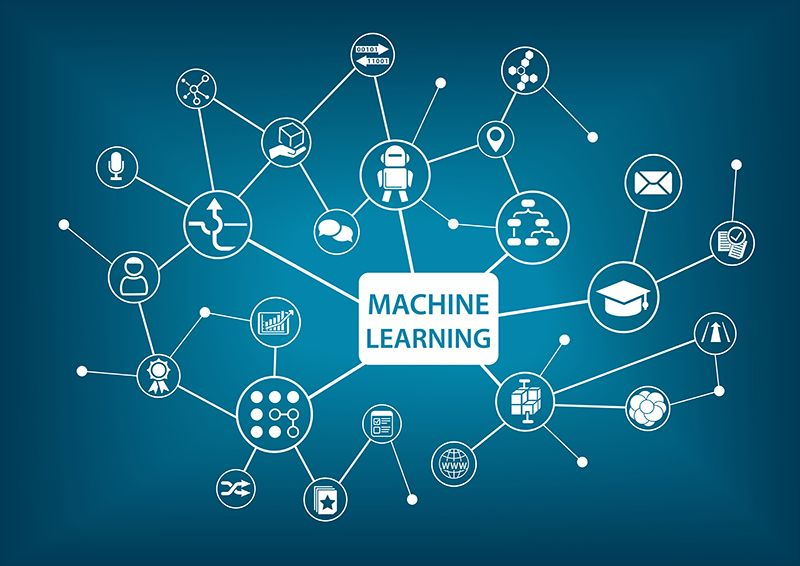
\includegraphics[width=0.65\textwidth]{ML.jpg}
	\caption[Machine Learning.]{Machine Learning.}
	\label{fig:ML}
\end{figure} 

Học máy được sử dụng rộng rãi trong nhiều lĩnh vực như xử lý ngôn ngữ tự nhiên, thị giác máy tính, nhận dạng giọng nói, dự đoán tín dụng và nhiều ứng dụng khác. Các phương pháp học máy phổ biến bao gồm học có giám sát, học không giám sát và học tăng cường.

\section{Tầm quan trọng của Machine Learning}

\begin{itemize}
	\item Học máy đóng vai trò rất quan trọng trong nhiều lĩnh vực bởi vì nó cung cấp cho chúng ta khả năng tự động hóa các tác vụ phức tạp và tối ưu hóa quy trình. 
	
	\item Xử lý các lượng dữ liệu lớn và phân tích chúng để tìm ra các mẫu và thông tin hữu ích.
	
	\item Cho phép dự đoán kết quả và đưa ra quyết định dựa trên tập dữ liệu đã học. Nhờ vào những ứng dụng của nó, học máy đã có ảnh hưởng to lớn đến nhiều lĩnh vực như y tế, tài chính, sản xuất, marketing, và nhiều lĩnh vực khác.
\end{itemize}

\section{Hệ thống nhận diện khẩu trang và cảm xúc}

Tuy dịch bệnh Covid 19 đã dần được đẩy lùi nhưng vẫn có nguy cơ bùng phát trở lại cùng với nhiều biến thể phức tạp. Bên cạnh đó, với sự xuất hiện nhiều loại bệnh lây truyền qua đường hô hấp đã thúc đẩy việc tạo ra những ứng dụng góp phần hỗ trợ việc phòng tránh bệnh, giúp cho người dân dễ dàng kiểm soát việc đeo khẩu trang đúng cách, giảm thiểu nguy cơ lây lan dịch bệnh trên diện rộng.

Việc áp dụng công nghệ Deep Learning vào bài toán nhận diện cảm xúc khuôn mặt và việc có hay không đeo khẩu trang đang được dự án triển khai và phát triển. Ứng dụng mô hình mạng nơ-ron tích chập (Convolutional Neural Network – CNN) được sử dụng rất nhiều trong lĩnh vực dự đoán hình ảnh. Trong báo cáo này, nhóm xây dựng một mô hình học máy sử dụng mô hình mạng tích chập CNN để nhận diện việc có hay không đeo khẩu trang cũng như kết hợp xây dựng mô hình nhận diện cảm xúc.

\section{Tổng quan bài toán} 

\subsection{Mô tả bài toán thực tế} 

\begin{itemize}
	\item Sử dụng mạng nơ-ron tích chập (CNN) huấn luyện một mô hình có thể nhận biết : Người có đeo khẩu trang , Không đeo khẩu trang và Đeo sai cách.
	
	\item Nếu không đeo khẩu trang thì có thể nhận biết cảm xúc cũng dùng mạng nơ-ron tích chập (CNN) để huấn luyện mô hình nhận dạng cảm xúc.
	
	\item Hệ thống camera để hiển thị lên màn hình trạng thái của việc đeo khẩu trang và cảm xúc.
\end{itemize}

\subsection{Mô tả bài toán chi tiết}

CNN hoạt động bằng cách sử dụng các bộ lọc (filters) để thực hiện phép tích chập (convolution) trên hình ảnh đầu vào. Bộ lọc này sẽ di chuyển trên toàn bộ hình ảnh, tìm kiếm các đặc trưng của hình ảnh bằng cách so sánh các khu vực nhỏ của hình ảnh với một mẫu được học trước. Các đặc trưng được tìm thấy sau đó sẽ được đưa vào một hoặc nhiều lớp ẩn để xử lý và trích xuất thông tin từ các đặc trưng này.

\begin{figure}[h!]
	\centering
	
\includegraphics[width=0.7\textwidth]{anh1.png}
	\caption[Quy trình huấn luyện ]{Quy trình huấn luyện}
	\label{fig:mohinh}
\end{figure} 

Sau khi thông tin được trích xuất, CNN sử dụng một số lớp Fully Connected (FC) để xử lý dữ liệu và cuối cùng đưa ra kết quả dự đoán về việc đeo có đeo khẩu trang không, đeo khẩu trang có đúng hay không.

Việc xây dựng một mô hình CNN cho chẩn đoán đeo khẩu trang yêu cầu một tập dữ liệu lớn về hình ảnh khuôn mặt, trong đó phải có đầy đủ các trường hợp đeo khẩu trang, không đeo khẩu trang, đeo khẩu trang sai cách cùng với tập ảnh về cảm xúc (angry, happy, neutral, fear, disgust,...). Sau đó, mô hình sẽ được huấn luyện trên tập dữ liệu này để học cách phân biệt các đặc trưng của hình ảnh đeo khẩu trang cũng như không đeo và đeo sai cách và cảm xúc khuôn mặt.



% Chương 2

\chapter{CƠ SỞ LÝ THUYẾT DÙNG ĐỂ GIẢI QUYẾT BÀI TOÁN} 

\label{Chapter2}

\section{Mạng neural tích chập (Convolutional Neural Network - CNN)}

\subsection{Khái niệm}

Mạng neural tích chập (Convolutional Neural Network - CNN) là một loại mạng neural sử dụng trong lĩnh vực xử lý ảnh và nhận dạng. Nó sử dụng các lớp tích chập để trích xuất đặc trưng từ ảnh đầu vào và áp dụng các lớp kết nối đầy đủ để phân loại ảnh. 

\begin{figure}[h!]
	\centering
	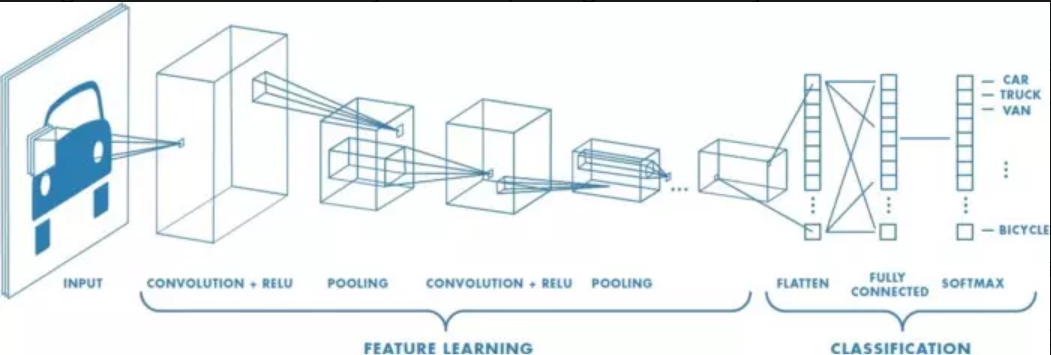
\includegraphics[width=0.8\textwidth]{CNN.png}
	\caption[Toàn bộ luồng CNN để xử lý hình ảnh đầu vào và phân loại các đối tượng dựa trên giá trị.]{Toàn bộ luồng CNN để xử lý hình ảnh đầu vào và phân loại các đối tượng dựa trên giá trị.}
	\label{fig:CNN} 
\end{figure}

Về kỹ thuật, mô hình CNN để training và kiểm tra, mỗi hình ảnh đầu vào sẽ chuyển nó qua 1 loạt các lớp tích chập với các bộ lọc (Kernel), tổng hợp lại các lớp được kết nối đầy đủ (Full Connected) và áp dụng hàm Softmax để phân loại đối tượng có giá trị xác suất giữa 0 và 1. Hình dưới đây là toàn bộ luồng CNN để xử lý hình ảnh đầu vào và phân loại các đối tượng dựa trên giá trị.

\begin{figure}[h!]
	\centering
	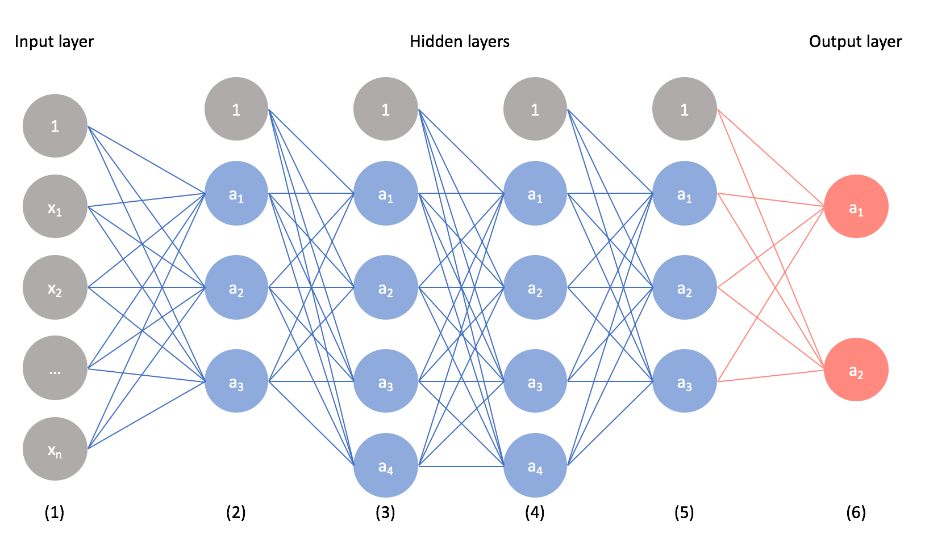
\includegraphics[width=0.7\textwidth]{anh2.png}
	\caption[Mô hình cấu trúc của mạng CNN.]{Mô hình cấu trúc của mạng CNN.}
	\label{fig:anh2} 
\end{figure}

\subsection{Feature trong CNN}

Các feature (đặc trưng) được sử dụng để trích xuất thông tin từ ảnh đầu vào. Các feature này được học tự động từ dữ liệu và được sử dụng để giảm thiểu số lượng thông tin cần xử lý trong quá trình huấn luyện mạng. 

Các feature này có thể là các đường cạnh, các vùng sáng tối, các đường cong và các đối tượng phức tạp hơn. 

Các feature này được trích xuất thông qua các bộ lọc tích chập và được kết hợp lại để tạo thành các feature maps, đóng vai trò quan trọng trong việc phân loại ảnh. Các feature maps này được đưa vào các lớp kết nối đầy đủ để phân loại ảnh đầu vào.

\subsection{Những lớp cơ bản của mạng CNN}

\subsubsection{Convolutional Layer}

Phần quan trọng nhất của toàn mạng CNN, các yếu tố quan trọng trong lớp Convolutional là: padding, stride, feature map và filter map.

\begin{itemize}
	\item Mạng CNN sử dụng filter để áp dụng vào các vùng của ma trận hình ảnh. Các filter map là các ma trận 3 chiều, bên trong đó là những tham số và chúng được gọi là parameters.
	
	\item Stride: dịch chuyển filter map theo từng pixel dựa vào các giá trị từ trái qua phải.
	
	\item Padding: Giá trị viền xung quanh của ma trận hình ảnh sẽ được gán các giá trị 0 để có thể tiến hành nhân tích chập ma trận mà không làm giảm kích thước ma trận ảnh ban đầu.
	
	\item Feature map: Biểu diễn kết quả sau mỗi lần feature map quét qua ma trận ảnh đầu vào. Sau mỗi lần quét thì lớp Convolutional sẽ tiến hành tính toán.
\end{itemize}

\begin{figure}[h!]
	\centering
	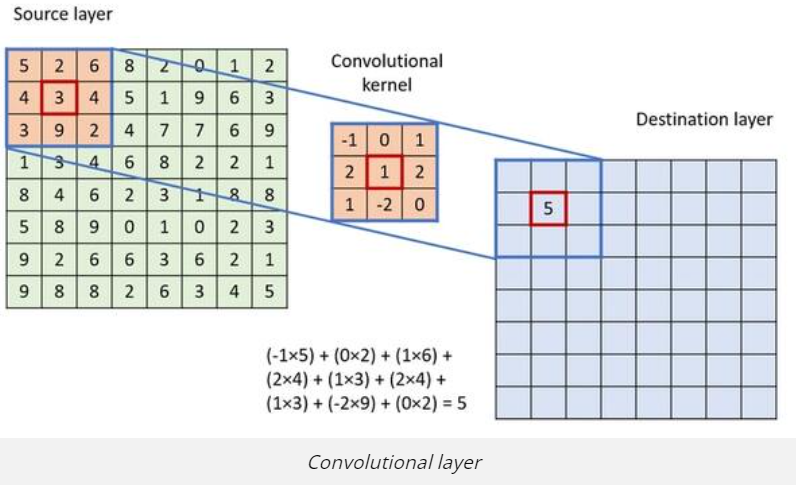
\includegraphics[width=0.7\textwidth]{convolution.png}
	\caption[Convolutional Layer.]{Convolutional Layer.}
	\label{fig:convolution} 
\end{figure}

\subsubsection{ReLU Layer}

Lớp ReLU là hàm kích hoạt trong mạng CNN, được coi là activation function. Nó có tác dụng mô phỏng những nơ ron có tỷ lệ truyền xung qua axon và hỗ trợ tính toán nhanh hơn.

Trong quá trình dùng hàm ReLU, chú ý đến việc tùy chỉnh learning rate và dead unit. Những lướp ReLU được dùng sau khi filter map được tính và áp dụng ReLU lên các giá trị của filter map.

\subsubsection{Pooling Layer}

Khi ma trận ảnh đầu vào có kích thước quá lớn, các lớp Pooling layer sẽ được đặt vào giữa những lớp Convolutional để làm giảm những parameters. Hai loại Pooling được sửu dụng phổ biến: Max pooling và Average.

\subsubsection{Fully Connected Layer}

Lớp có nhiệm vụ đưa ra kết quả sau khi 2 lớp Convolutional và Pooling đã nhận được ảnh truyền, khi này, ta sẽ thu được một model đọc được thông tin của ảnh.

\subsection{Kiến trúc của mạng CNN}

Mạng CNN là tập hợp những Convolutional layer xếp chồng lên nhau, đồng thời mạng sử dụng những hàm như ReLU và Tanh để kích hoạt các trọng số trong các node. Các lớp này sau khi qua các hàm activation sẽ có trọng số trong những node và có thể tạo ra những thông tin trừu tượng hơn đến với các lớp kế tiếp trong mạng.  

Cấu trúc cơ bản của một mô hình CNN:

\begin{itemize}
	\item Local receptive: Lớp này sử dụng để tách lọc dữ liệu, thông tin hình ảnh để từ đó có thể lựa chọn các vùng có giá trị sử dụng hiệu quả cao nhất.
	
	\item Shared weights field: Lớp này hỗ trợ làm giảm các tham số đến mức tối thiểu trong mạng CNN. Trong từng lớp convolution sẽ chứa các feature map riêng và từng feature thì sẽ có khả năng phát hiện một vài feature trong hình ảnh.
	
	\item Pooling layer: Lớp cuối cùng và sử dụng để làm đơn giản các thông tin output. Sau khi tính toán xong và quét qua các layer trong mạng thì pooling layer sẽ được dùng để lược bỏ các thông tin không hữu ích.
\end{itemize}

\section{Các thư viện được sử dụng}

\subsubsection{Thư viện Numpy}

Thư viện NumPy (Numerical Python) là một thư viện Python phổ biến được sử dụng để làm việc với mảng đa chiều và các phép toán số học trên chúng. NumPy cung cấp một cấu trúc dữ liệu mảng mạnh mẽ và các hàm tiện ích để thực hiện các phép toán số học, xử lý mảng và thao tác trên dữ liệu số.

Dưới đây là một số khái niệm và tính năng chính của NumPy:

\begin{itemize}
	\item Mảng NumPy (ndarray): Mảng NumPy là cấu trúc dữ liệu chính trong NumPy, cho phép lưu trữ và xử lý các mảng đa chiều. Mảng NumPy có kích thước cố định và các phần tử trong mảng cùng kiểu dữ liệu.
	
	\item Các phép toán số học: NumPy cung cấp các hàm và toán tử cho phép thực hiện các phép toán số học trên mảng như cộng, trừ, nhân, chia, lũy thừa, căn bậc hai, logarit...
	
	\item Truy cập phần tử: Bạn có thể truy cập và thay đổi giá trị các phần tử trong mảng NumPy bằng cách sử dụng chỉ mục và cắt mảng (slicing).
	
	\item Hàm toán học và thống kê: NumPy cung cấp nhiều hàm toán học và thống kê tiện ích như min, max, mean, sum, std,... để thao tác trên mảng.
	
	\item Hàm điều kiện: NumPy cung cấp các hàm và phương thức cho phép kiểm tra và lựa chọn các phần tử trong mảng dựa trên các điều kiện như np.where, np.logical$\_$and, np.logical$\_$or,...
	
	\item Thao tác trên mảng: NumPy cung cấp các hàm và phương thức để thực hiện các phép biến đổi mảng như reshape, transpose, flatten, concatenate,...
	
	\item Tích hợp C/C++: NumPy cho phép tích hợp mã C/C++ vào mã Python thông qua giao diện C API của nó, giúp tăng tốc độ xử lý các phép toán số học.
	
	\item NumPy được sử dụng rộng rãi trong nhiều lĩnh vực như khoa học dữ liệu, máy học, tính toán khoa học, xử lý ảnh và âm thanh, mô phỏng vật lý,... Thư viện này là một phần quan trọng của hệ sinh thái Python cho tính toán số và xử lý dữ liệu.
\end{itemize}

\subsubsection{Thư viện OpenCV}

Thư viện cv2 (OpenCV) là một thư viện mã nguồn mở được sử dụng rộng rãi trong xử lý ảnh và thị giác máy tính trong ngôn ngữ lập trình Python. OpenCV cung cấp nhiều chức năng và công cụ mạnh mẽ để xử lý, phân tích và trực quan hóa ảnh và video. Dưới đây là một số chức năng chính của thư viện cv2:

\begin{itemize}
	\item Đọc và ghi ảnh và video: OpenCV cung cấp các hàm để đọc và ghi các tệp tin ảnh và video từ các nguồn khác nhau, bao gồm ổ đĩa, camera,...
	
	\item Xử lý ảnh: OpenCV cung cấp nhiều chức năng để xử lý ảnh, bao gồm chuyển đổi màu sắc, cắt, xoay, thu phóng, lật, v.v. Bạn cũng có thể áp dụng các bộ lọc, làm mờ, lọc nhiễu, phát hiện cạnh và nhiều phép biến đổi khác cho ảnh.
	
	\item Xử lý video: OpenCV hỗ trợ xử lý video, bao gồm khung hình theo thời gian, trích xuất khung hình, ghi lại video và áp dụng các hiệu ứng video.
	
	\item Xử lý thị giác máy tính: OpenCV cung cấp các chức năng và thuật toán để phân tích và nhận dạng các đối tượng trong ảnh, bao gồm nhận dạng khuôn mặt, phát hiện vật thể, trích xuất đặc trưng, theo dõi đối tượng,...
	
	\item Xử lý điểm ảnh: OpenCV cho phép bạn truy cập và chỉnh sửa các điểm ảnh trực tiếp, bao gồm xử lý pixel, tạo hiệu ứng đồ họa và thực hiện các phép tính điểm ảnh phức tạp.
	
	\item Hiển thị ảnh: OpenCV cung cấp các chức năng để hiển thị ảnh và video trực tiếp trên màn hình, tạo cửa sổ đồ họa và tương tác với ảnh.
\end{itemize}

Thư viện cv2 có tính ổn định, tốc độ xử lý nhanh và rất phổ biến trong cộng đồng xử lý ảnh và thị giác máy tính.

\subsubsection{Thư viện Tensorflow}

Thư viện TensorFlow là một thư viện mã nguồn mở phát triển bởi Google AI và được sử dụng rộng rãi trong lĩnh vực học máy và trí tuệ nhân tạo. TensorFlow cung cấp một cấu trúc dữ liệu gọi là "đồ thị tính toán" (computational graph) để biểu diễn và thực thi các phép tính toán số trên dữ liệu. Đồ thị tính toán trong TensorFlow bao gồm các nút (nodes) đại diện cho các phép tính toán và các cung (edges) đại diện cho luồng dữ liệu giữa các nút. Dưới đây là một số khái niệm và tính năng chính của TensorFlow:

\begin{itemize}
	\item Đồ thị tính toán (Computational graph): TensorFlow sử dụng đồ thị tính toán để biểu diễn và thực thi các phép tính toán. Đồ thị tính toán giúp tối ưu hóa và tận dụng được tính song song của phần cứng để thực hiện các phép tính nhanh chóng.
	
	\item Tensors: TensorFlow sử dụng cấu trúc dữ liệu tensor để lưu trữ và xử lý dữ liệu. Tensor có thể là một vector, ma trận, hay một mảng đa chiều với các phần tử cùng kiểu dữ liệu.
	
	\item Các lớp và phép tính: TensorFlow cung cấp một loạt các lớp và phép tính để xây dựng các mô hình học máy. Các lớp bao gồm các lớp mạng nơ-ron, lớp tích chập, lớp tổng hợp, lớp tái tạo,... Phép tính bao gồm các phép tính toán như cộng, trừ, nhân, chia, lũy thừa,...
	
	\item Tối ưu hóa và tạo mô hình: TensorFlow cung cấp các tối ưu hóa để tối đa hóa hiệu suất và tăng tốc độ huấn luyện mô hình. Ngoài ra, TensorFlow cũng cung cấp khả năng tạo và lưu trữ các mô hình đã huấn luyện để sử dụng sau này.
	
	\item Tích hợp và mở rộng: TensorFlow cho phép tích hợp và mở rộng với các công cụ và thư viện khác như Keras, scikit-learn, OpenCV, v.v. Điều này giúp thực hiện các tác vụ phức tạp và kết hợp các công cụ và thuật toán khác nhau.
	
	\item Tính tương thích và di động: TensorFlow hỗ trợ nhiều phiên bản và cung cấp tính tương thích đa nền tảng, cho phép chạy trên các thiết bị di động, máy tính cá nhân, máy chủ, và cụm máy tính phân tán.
\end{itemize}

TensorFlow là một công cụ mạnh mẽ trong lĩnh vực học máy và trí tuệ nhân tạo, cho phép xây dựng và huấn luyện các mô hình phức tạp và giải quyết các bài toán thực tế.

\subsubsection{Thư viện Sklearn}

Scikit-learn, hay còn được gọi là sklearn, là một thư viện mã nguồn mở phổ biến trong ngôn ngữ lập trình Python được sử dụng cho Machine Learning và Data Mining. Scikit-learn cung cấp nhiều công cụ và thuật toán tiện ích để xây dựng và đánh giá các mô hình học máy, phân tích dữ liệu và thực hiện các tác vụ tiền xử lý dữ liệu. Dưới đây là một số chức năng và tính năng chính của thư viện scikit-learn:

\begin{itemize}
	\item Cung cấp các thuật toán học máy tiêu chuẩn: Scikit-learn cung cấp các thuật toán học máy phổ biến như hồi quy tuyến tính, hồi quy logistic, máy vector hỗ trợ (SVM), cây quyết định, Random Forest, K-means clustering,... Các thuật toán này được triển khai một cách hiệu quả và dễ sử dụng.
	
	\item Tích hợp các công cụ tiền xử lý dữ liệu: Scikit-learn cung cấp nhiều công cụ tiền xử lý dữ liệu như chuẩn hóa dữ liệu, mã hóa biến định danh, xử lý giá trị thiếu, trích xuất đặc trưng,... Điều này giúp chuẩn bị dữ liệu cho việc huấn luyện mô hình.
	
	\item Đánh giá và tối ưu hóa mô hình: Scikit-learn cung cấp các phép đo và công cụ để đánh giá hiệu suất của mô hình học máy, bao gồm chia dữ liệu thành tập huấn luyện và tập kiểm tra, cross-validation, tính toán độ chính xác, độ phân loại, mất mát,... Ngoài ra, scikit-learn cũng cung cấp các công cụ tối ưu hóa để điều chỉnh các siêu tham số của mô hình.
	
	\item Tích hợp với các thư viện khác: Scikit-learn tích hợp tốt với các thư viện khác trong hệ sinh thái của Python như NumPy, Pandas và Matplotlib, tạo điều kiện thuận lợi cho xử lý dữ liệu và trực quan hóa kết quả.
\end{itemize}

Scikit-learn là một công cụ mạnh mẽ và phổ biến trong lĩnh vực Machine Learning, đặc biệt là trong các tác vụ phân loại, hồi quy và gom cụm dữ liệu. Với tư cách là một thư viện mã nguồn mở, scikit-learn đang tiếp tục được phát triển và cung cấp cập nhật mới để phục vụ cộng đồng Machine Learning ngày càng lớn.

\subsubsection{Thư viện Matplotlib}

Matplotlib là một thư viện trong Python được sử dụng để tạo và hiển thị đồ thị, biểu đồ, hình ảnh và các loại visualizations khác. Nó cung cấp các công cụ mạnh mẽ để tạo ra các biểu đồ chất lượng cao, giúp bạn trực quan hóa dữ liệu một cách dễ dàng và linh hoạt. Dưới đây là một số thành phần chính trong thư viện matplotlib:

\begin{itemize}
	\item pyplot: Giao diện API cơ bản của Matplotlib, cung cấp các hàm để tạo và tùy chỉnh đồ thị và biểu đồ.
	
	\item Figure: Đại diện cho một hình ảnh hoặc một tệp tin hình ảnh.
	
	\item Axes: Cung cấp các phương thức để tạo các đối tượng đồ thị như các trục, điểm, đường.
	
	\item Subplots: Cho phép tạo và quản lý nhiều đồ thị trong cùng một hình ảnh.
	
	\item Plot: Hàm để tạo các loại đồ thị và biểu đồ, bao gồm đồ thị đường (line plot), biểu đồ cột (bar plot), biểu đồ hộp (box plot), đồ thị điểm (scatter plot).
	
	\item Colorbar: Hiển thị thanh màu để giải thích giá trị của màu sắc trong đồ thị.
	
	\item Title, Label, Legend`: Cung cấp các phương thức để thêm tiêu đề, nhãn và chú giải vào đồ thị.
\end{itemize}

Matplotlib cũng hỗ trợ nhiều kiểu đồ thị và biểu đồ, cho phép bạn tùy chỉnh màu sắc, kích thước, kiểu đường, điểm, các đánh dấu trục, v.v. Thư viện này rất linh hoạt và mạnh mẽ, cho phép bạn tạo ra các visualizations phức tạp và tùy chỉnh chúng theo ý muốn.

\subsubsection{Thư viện Keras}

Keras là một thư viện mã nguồn mở cho Python được sử dụng để xây dựng các mô hình học máy và mạng nơ-ron. Nó được thiết kế để làm cho việc xây dựng mô hình học máy trở nên dễ dàng và nhanh chóng hơn. Keras có nhiều tính năng hữu ích, bao gồm:

\begin{itemize}
	\item Dễ dàng sử dụng: Keras được thiết kế để làm cho việc xây dựng mô hình học máy trở nên dễ dàng và trực quan hơn.
	
	\item Tích hợp với các thư viện tính toán số: Keras hỗ trợ các thư viện tính toán số như TensorFlow, Theano và CNTK, cho phép bạn chọn thư viện tính toán số phù hợp nhất cho dự án của mình.
	
	\item Hỗ trợ nhiều loại mô hình: Keras hỗ trợ nhiều loại mô hình, bao gồm mạng nơ-ron tiêu chuẩn, mạng nơ-ron tích chập và mạng nơ-ron tái tạo.
	
	\item Tích hợp với các công cụ tối ưu hóa: Keras cung cấp các công cụ tối ưu hóa để giúp bạn tìm kiếm các tham số tốt nhất cho mô hình của mình.
	
	\item Hỗ trợ các lớp và hàm kích hoạt tiêu chuẩn: Keras cung cấp các lớp và hàm kích hoạt tiêu chuẩn để giúp bạn xây dựng mô hình học máy nhanh chóng và dễ dàng.
\end{itemize}

Keras là một trong những thư viện phổ biến nhất cho việc xây dựng các mô hình học máy và mạng nơ-ron. 

\section{Mô hình phát hiện khuôn mặt}

Việc sử dụng mô hình phát hiện khuôn mặt có sẵn như ResnetSSD là một cách tiếp cận hiệu quả để nhận dạng và phát hiện khuôn mặt trong các ứng dụng thực tế. Mô hình này được xây dựng trên nền tảng deep learning và có khả năng phát hiện khuôn mặt với độ chính xác cao.

Một số lưu ý khi sử dụng mô hình này là:

\begin{itemize}
	\item Đảm bảo rằng ảnh hoặc video đầu vào đủ lớn và độ phân giải cao để đảm bảo độ chính xác của kết quả phát hiện.
	
	\item Có thể cần điều chỉnh các tham số của mô hình để phù hợp với ứng dụng cụ thể.
	
	\item Để đạt được hiệu quả cao nhất, nên sử dụng mô hình này kết hợp với các công cụ nhận dạng khuôn mặt khác để xác định danh tính của người được phát hiện.
\end{itemize}

Với mô hình phát hiện khuôn mặt ResnetSSD, bạn có thể dễ dàng tích hợp vào các ứng dụng thực tế như hệ thống an ninh, ứng dụng nhận dạng khuôn mặt và nhiều ứng dụng khác.

Trong đề tài này, chúng ta sử dụng một mô hình phát hiện khuôn mặt có sẵn để có thể phát hiện khuôn mặt, từ đó chúng ta có thể dự đoán việc đeo khẩu trang và nhận diện cảm xúc.









 
% Chương 3

\chapter{CHƯƠNG TRÌNH THỰC NGHIỆM} 

\label{Chapter3} 

\section{Bộ dữ liệu}

Bộ dữ liệu hình ảnh được lấy từ: \href{https://www.kaggle.com/datasets/spandanpatnaik09/face-mask-detectormask-not-mask-incorrect-mask}{Kaggle} 

*** Dữ liệu mask và Dữ liệu cảm xúc (emotion)

\begin{figure}[h!] 
	\begin{tabular}{cc}
		\centering
		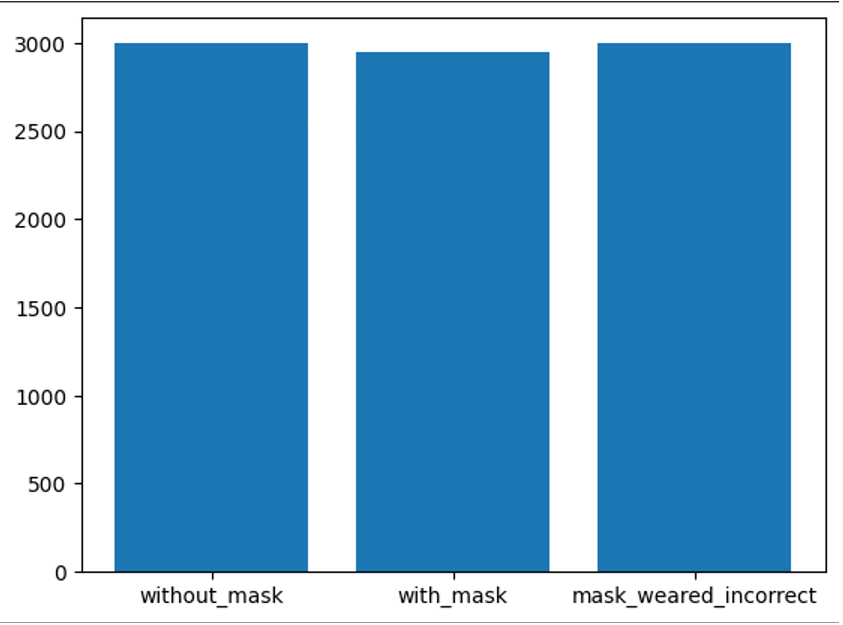
\includegraphics[width=0.5\textwidth]{mask.png} &
		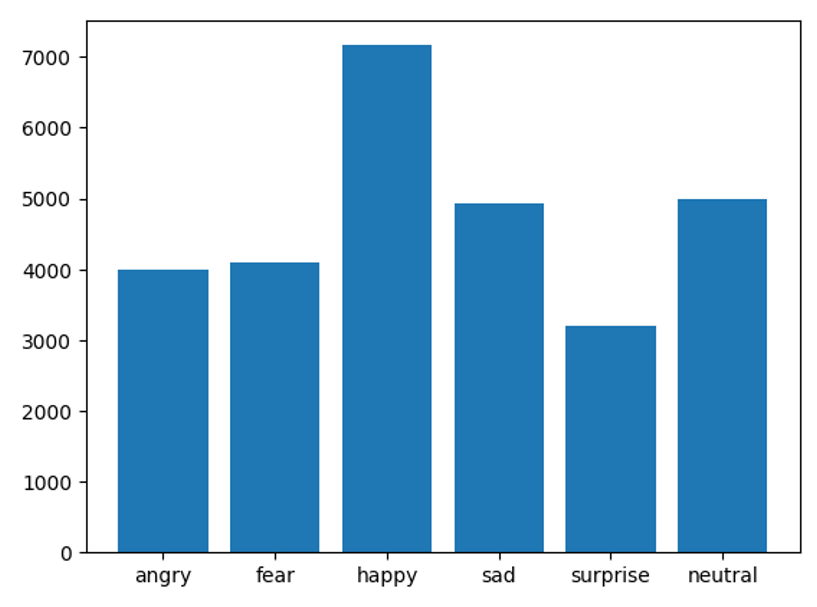
\includegraphics[width=0.5\textwidth]{emotion.png} 
	\end{tabular}
	\caption[Bộ dữ liệu mask và emotion.]{Bộ dữ liệu mask và emotion.}
	\label{fig:maskemotion}
\end{figure}

\section{Chỉ số đánh giá hiệu suất}

Để đánh giá phân loại ảnh được chính xác, các mô hình trong phần trước sữ được chạy bằng cách sử dụng bộ dữ liệu dưới dạng hình ảnh, vì vậy cần có sự điều chỉnh để nâng cấp độ chính xác của chúng. Đối với mỗi mô hình 3 kết quả điển hình được hiển thị trong CNN là:

\begin{itemize}
	\item Đồ thị độ chính xác (model ACC): ACC cho biết sự thay đổi độ chính xác của mô hình qua các vòng lặp/epochs trong quá trình huấn luyện.
	
	\item Đồ thị loss (model loss): Đồ thị loss biểu thị sự thay đổi của hàm loss của mô hình qua các vòng lặp hoặc epochs trong quá trình huấn luyện. Hàm loss tính toán sự sai khác giữa giá trị dự đoán của mô hình và giá trị thực tế.
	
	\item Confusion matrix: Về cơ bản, Confusion matrix thể hiện có bao nhiêu điểm dữ liệu thực sự thuộc vào một class, và được dự đoán là rơi vào một class. 
	
	\begin{figure}[h!]
		\centering
		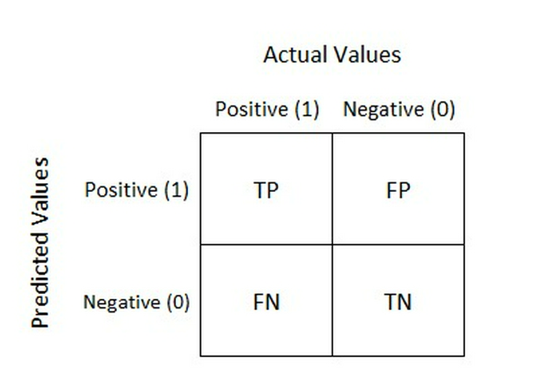
\includegraphics[width=0.7\textwidth]{cofusion.png}
		\caption[Confusion matrix.]{Confusion matrix.}
		\label{fig:cm} 
	\end{figure}

	\begin{itemize}
		\item TP (True Positive): Số lượng dự đoán chính xác.
		
		\item TN (True Negative): Số lương dự đoán chính xác một cách gián tiếp. Là khi mô hình dự đoán đúng một người không bị bệnh tức là việc không chọn trường hợp bị bệnh là chính xác.
		
		\item FP (False Positive - Type 1 Error): Số lượng các dự đoán sai lệch. Là khi mô hình dự đoán một người bị bệnh và người đó hoàn toàn khỏe mạnh.
		
		\item FN (False Negative - Type 2 Error): Số lượng các dự đoán sai lệch một cách gián tiếp. Là khi mô hình dự đoán một người không bị bệnh nhưng người đó bị bệnh, tức là việc không chọn trường hợp bị bệnh là sai. 		
	\end{itemize}
	$\Longrightarrow$ Từ 4 chỉ số TP, TN, FP, FN, ta có 4 chỉ số để đánh giá mức độ tin cậy của một mô hình:
\end{itemize}

\begin{itemize}
	\item Accuracy: Được tính bằng cách chia tổng số dự đoán đúng cho tất cả các dự đoán.
	
	\begin{figure}[h!]
		\centering
		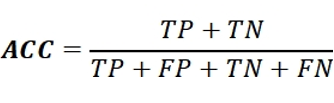
\includegraphics[width=0.45\textwidth]{acc1.png}
		\caption[Accuracy.]{Accuracy.}
		\label{fig:acc} 
	\end{figure}
		
	\item Precision: Trong tất cả các dự đoán Positive được đưa ra, bao nhiêu dự đoán là chính xác.
	
	\begin{figure}[h!]
		\centering
		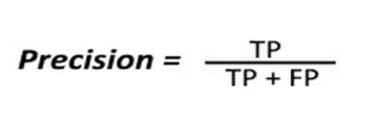
\includegraphics[width=0.6\textwidth]{precision.png}
		\caption[Precision.]{Precision.}
		\label{fig:precision} 
	\end{figure}
	
	\item Recall: Trong tất cả các trường hợp Positive, bao nhiêu trường hợp đã được dự đoán chính xác.		
	
	\begin{figure}[h!]
		\centering
		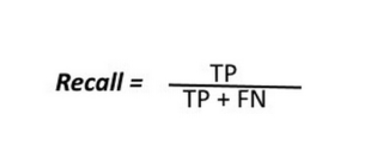
\includegraphics[width=0.6\textwidth]{recall.png}
		\caption[Recall.]{Recall.}
		\label{fig:recall} 
	\end{figure}

	\item F1-Score: Dùng để đánh giá mức độ tin cậy chung của mô hình
	
	\begin{figure}[h!]
		\centering
		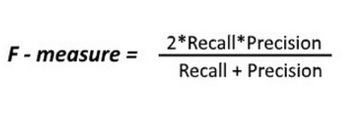
\includegraphics[width=0.6\textwidth]{score.png}
		\caption[F1-Score.]{F1-Score.}
		\label{fig:score} 
	\end{figure}
\end{itemize}

\section{Huấn luyện mô hình và kết quả thực nghiệm}

Do các bước tiền xử lý dữ liệu của 2 mô hình là như nhau thế nên trong báo cáo này em chỉ trình bày cách nhóm em xử lý dữ liệu của bộ dự hiệu khẩu trang.

\subsection{Tiền xử lý dữ liệu} 

*** Import một số thư viện để xử lí và phân tích trực quan dữ liệu:

\begin{lstlisting}[style=codePython]
  	import glob
  	import shutil
  	import cv2 
  	from PIL import Image
  	import PIL
  	import os
  	import numpy as np
  	import pandas as pd
  	import matplotlib.pyplot as plt
  	import seaborn as sns
  	import random 
  	from sklearn.model_selection import train_test_split
  	import tensorflow as tf
  	import keras
  	from keras.preprocessing import image
  	from keras.models import Sequential
  	from keras.layers import Conv2D, MaxPool2D, Flatten,Dense,Dropout,BatchNormalization
  	from keras import regularizers

  	import warnings
  	# Ignore waring
  	warnings.filterwarnings('ignore')  	
\end{lstlisting}

*** Tiền xử lý dữ liệu: 

\begin{itemize}
	\item Tiền xử lý dữ liệu là một bước rất quan trọng trong việc giải quyết bất kỳ vấn đề nào trong lĩnh vực học máy. Hầu hết các bộ dữ liệu được sử dụng trong các vấn đề liên quan đến học máy cần được xử lý, làm sạch và biến đổi trước khi một thuật toán có thể được huấn luyện trên những bộ dữ liệu này.
	
	\item Load dữ liệu hình ảnh vào tập train và labels.
	
	\begin{itemize}
		\item Tạo đường dẫn:
		
		\begin{lstlisting}[style=codePython]
			mask_path = ['/without_mask/*','/with_mask/*','/incorrect_mask/*' ]
			
			train_path = '/content/drive/MyDrive/Dataset/processed'			
		\end{lstlisting}
		
		\item Load dữ liệu:
		
		\begin{lstlisting}[style=codePython]
			X = []
			y = []
			for i, path in enumerate(mask_path):
			for name in glob.glob(train_path + path):
			img = cv2.imread(name)
			img = cv2.cvtColor(img,cv2.COLOR_BGR2RGB)
			img = cv2.resize(img,(48,48))
			X.append((img))
			y.append(i)
			len(X)					
		\end{lstlisting}
	
		\item Chuẩn hóa dữ liệu hình ảnh: Các giá trị pixel được đưa về các giá trị trong khoảng từ 0 đến 1 giúp mô hình học tốt hơn.
		
		\begin{lstlisting}[style=codePython]
			X = np.array(X)/255.
			y = np.array(y)			
		\end{lstlisting}
	
		\item Phân tích dữ liệu thành tập train và tập test: Sau đó ta tạo 4 biến, gồm X$\_$train, y$\_$train và X$\_$test, y$\_$test. Với đối số truyền vào là giá trị X, y ta đã lấy từ dữ liệu bên trên, test$\_$size trả về cho ta phần trăm dữ liệu được chia, ví dụ 0.2 tương ứng với dữ liệu được chia thành 20\% giá trị là test, còn lại là dữ liệu train. random$\_$state bằng một số tương ứng nào đó để đảm bảo mỗi lần ta chạy lại mô hình, giá trị phân tách ngẫu nhiên nhận được là giống nhau, bạn có thể cho số nào bất kỳ. 
		
		 \begin{lstlisting}[style=codePython]
		 	X_train, X_test, y_train, y_test = train_test_split(X, y, test_size=0.2, random_state=2)			
		 \end{lstlisting}
	 
	 	\item Chuẩn hóa dữ liệu output: Chuyển về dạng onehot để phân biệt nhiều ảnh một cách dễ dàng  
	 	
	 	\begin{lstlisting}[style=codePython]
	 		from sklearn.preprocessing import OneHotEncoder
	 		encoder = OneHotEncoder()
	 		encoder.fit(y_train.reshape(-1,1))
	 		y_train = encoder.transform(y_train.reshape(-1,1)).toarray()
	 		y_test = encoder.transform(y_test.reshape(-1,1)).toarray()
	 		print(y_train) 				
	 	\end{lstlisting}		
	\end{itemize}
\end{itemize} 

\subsection{Mô hình huấn luyện CNN}

\subsubsection{Mô hình nhận dạng khẩu trang}

\begin{lstlisting}[style=codePython]
	inp = Input(shape = (48,48,3))
	cnn = Conv2D(filters =16,kernel_size = 3,activation ='relu')(inp)
	pooling = MaxPooling2D(pool_size =(2,2))(cnn)
	drop = Dropout(0.2)(pooling)
	
	cnn = Conv2D(filters =32,kernel_size = 3,activation ='relu')(inp)
	pooling = MaxPooling2D(pool_size =(2,2))(cnn)
	drop = Dropout(0.2)(pooling)
	
	cnn = Conv2D(filters =64,kernel_size = 4,activation ='relu')(inp)
	pooling = MaxPooling2D(pool_size =(2,2))(cnn)
	drop = Dropout(0.2)(pooling)
	
	cnn = Conv2D(filters =128, kernel_size =4,activation ='relu')(drop)
	pooling = MaxPooling2D(pool_size =(2,2))(cnn)
	drop = Dropout(0.2)(pooling)
	
	f =Flatten()(pooling)
	
	fc1 = Dense(units =128, activation ='relu')(f)
	fc2 = Dense(units =64, activation ='relu')(fc1)
	fc3 = Dense(units =32, activation ='relu')(fc2)
	out = Dense(units =3, activation ='softmax')(fc3)
	
	model =Model(inputs = inp,outputs =out)
	model.summary()	 				
\end{lstlisting}

$\Longrightarrow$ Đoạn code này định nghĩa một mô hình mạng neural tích chập (CNN) để phân loại ảnh với ba lớp đầu ra. 

\begin{itemize}
	\item Biến inp định nghĩa một hình dạng đầu vào là 48x48 pixel với 3 kênh màu (RGB).
	
	\item Sau đó là 4 lớp tích chập (Conv2D) với số lượng bộ lọc, kích thước kernel và kích hoạt ReLU tăng dần. Lớp đệm padding để giữ nguyên kích thưởng đầu ra. Mỗi lớp tích chập được theo sau bởi một lớp giảm kích thước (MaxPooling2D) để giảm kích thước không gian của đầu ra từ lớp tích chập. Các lớp giảm kích thước này giúp giảm thiểu quá khớp và cải thiện tốc độ và hiệu suất. Mỗi lớp giảm kích thước cũng được theo sau bởi một lớp dropout (Dropout) với tỷ lệ 0.2, loại bỏ ngẫu nhiên 20\% của các neuron để giảm thiểu quá khớp.
	
	\item Sau các lớp tích chập và giảm kích thước, đầu ra đã được làm phẳng từ lớp giảm kích thước cuối cùng, được đưa vào ba lớp kết nối đầy đủ (Dense) với số lượng đơn vị giảm dần và kích hoạt ReLU. Lớp đầu ra có 3 đơn vị với hàm kích hoạt softmax, xuất ra xác suất lớp cho mỗi ảnh đầu vào.
	
	\item Mô hình được tạo ra bằng cách sử dụng hàm Model từ Keras, với lớp đầu vào và đầu ra được xác định là inp và out, tương ứng.
	
	\item Cuối cùng, hàm model.summary() được sử dụng để in ra tóm tắt kiến trúc mô hình, bao gồm các loại lớp, hình dạng và số lượng tham số.
\end{itemize}

*** Sau khi đã xây dựng được kiến trúc của mô hình . Bước tiếp theo là thực hiện huấn luyện mô hình: 

\begin{lstlisting}[style=codePython]
	optimizer1 = tensorflow.keras.optimizers.Adam(learning_rate = 0.0001)
	model.compile(optimizer = optimizer1, loss = 'categorical_crossentropy',metrics =['accuracy'])
	
	history = model.fit(X_train,y_train,batch_size =16, epochs =25,validation_data =(X_test,y_test))				
\end{lstlisting}

\subsubsection{Mô hình nhận dạng cảm xúc}

\begin{lstlisting}[style=codePython]
	model= tf.keras.models.Sequential()
	model.add(Conv2D(32, kernel_size=(3, 3), padding='same', activation='relu', input_shape=(48, 48,1)))
	model.add(Conv2D(64,(3,3), padding='same', activation='relu' ))
	model.add(BatchNormalization())
	model.add(MaxPool2D(pool_size=(2, 2)))
	model.add(Dropout(0.25))
	
	model.add(Conv2D(128,(5,5), padding='same', activation='relu'))
	model.add(BatchNormalization())
	model.add(MaxPool2D(pool_size=(2, 2)))
	model.add(Dropout(0.25))
	
	model.add(Conv2D(512,(3,3), padding='same', activation='relu', kernel_regularizer=regularizers.l2(0.01)))
	model.add(BatchNormalization())
	model.add(MaxPool2D(pool_size=(2, 2)))
	model.add(Dropout(0.25))
	
	model.add(Conv2D(512,(3,3), padding='same', activation='relu', kernel_regularizer=regularizers.l2(0.01)))
	model.add(BatchNormalization())
	model.add(MaxPool2D(pool_size=(2, 2)))
	model.add(Dropout(0.25))
	
	model.add(Flatten()) 
	model.add(Dense(256,activation = 'relu'))
	model.add(BatchNormalization())
	model.add(Dropout(0.25))
	
	model.add(Dense(512,activation = 'relu'))
	model.add(BatchNormalization())
	model.add(Dropout(0.25))
	
	model.add(Dense(6, activation='softmax'))
	model.summary()					
\end{lstlisting}

$\Longrightarrow$ Đây là một mô hình CNN (Convolutional Neural Network) có kiến trúc phức tạp. Mô hình bao gồm 5 lớp tích chập (Conv2D) với các bộ lọc kích thước khác nhau và hàm kích hoạt là ReLU.

\begin{itemize}
	\item Lớp đầu tiên có 32 bộ lọc kích thước 3x3, lớp thứ hai có 64 bộ lọc kích thước kernel 3x3, lớp thứ ba là lớp có 128 bộ lọc  kích thước 5x5 và lớp cuối cùng là 2 lớp với 512 bộ lọc kích thước 3x3 và kết hợp với hàm chính quy (regularization) để giúp mô hình tránh overfitting.
	
	\item Sau mỗi lớp tích chập, model sử dụng một lớp BatchNormalization để chuẩn hóa giá trị và tăng tốc độ hội tụ. Lớp MaxPool2D được sử dụng để giảm kích thước của đầu ra và giảm số lượng tham số của mô hình. Lớp Dropout được sử dụng để giảm hiện tượng overfitting.
	
	\item Cuối cùng, một lớp Dense với 256 đơn vị và hàm kích hoạt ReLU được thêm vào mô hình, sau đó theo sau bởi một lớp Dropout và BatchNormalization. Sau đó, một lớp Dense với 512 đơn vị và hàm kích hoạt ReLU được chỉ định kế tiếp và kết thúc bằng lớp Dense với 6 đơn vị đầu ra với hàm kích hoạt soft$\_$max (6 lớp tương ứng với 6 cảm xúc).
	\item Mô hình được tạo ra bằng cách sử dụng hàm Model từ Keras, với lớp đầu vào và đầu ra được xác định là inp và out, tương ứng.
	
	\item Cuối cùng, hàm model.summary() được sử dụng để in ra tóm tắt kiến trúc mô hình, bao gồm các loại lớp, hình dạng và số lượng tham số.
\end{itemize}

*** Sau khi đã xây dựng được kiến trúc của mô hình . Bước tiếp theo là thực hiện huấn luyện mô hình: 

\begin{lstlisting}[style=codePython]
	learning_rate = 0.0001
	optimizer1 = tf.keras.optimizers.Adam(learning_rate = 0.0001)
	
	model.compile(optimizer = optimizer1, loss = 'categorical_crossentropy',metrics =['accuracy'])
	
	history = model.fit(X_train, y_train, epochs=40,validation_data=(X_test_scaled, y_test),batch_size = 64,shuffle = True)					
\end{lstlisting}

*** Từ bước huấn luyện mô hình, ta có: 

\begin{itemize}
	\item optimizer1: Optimizer được khởi tạo bằng cách sử dụng Adam optimizer từ tensorflow.keras.optimizers, với learning$\_$rate = 0.0001
	
	\item model.compile(): Cấu hình mô hình với optimizer, hàm mất mát là categotical$\_$crossentropy và các metric là accuracy để đánh giá hiệu suất mô hình.
	
	\item model.fit(): Huấn luyện mô hình trên dữ liệu huấn luyện (X$\_$train, y$\_$train) với các tham số như batch$\_$size, epochs, và sử dụng dữ liệu kiểm tra (X$\_$test, y$\_$test) để đánh giá hiệu suất của mô hình trong quá trình huấn luyện.
\end{itemize}

\subsection{Tiêu chí ảnh hưởng đến mô hình}	

Có nhiều yếu tố ảnh hưởng đến độ hiệu quả của một mô hình máy học. Dưới đây là một số tiêu chí quan trọng:

\begin{itemize}
	\item Độ rõ ràng và độ phong phú của dữ liệu: Mô hình sẽ hoạt động tốt hơn khi dữ liệu huấn luyện rõ ràng, có độ phân loại cao và đủ đa dạng. Dữ liệu không rõ ràng, nhiễu và thiếu thông tin có thể làm giảm độ hiệu quả của mô hình.
	
	\item Số lượng và chất lượng dữ liệu: Một số lượng dữ liệu huấn luyện đủ lớn có thể giúp mô hình học được các mẫu và mối quan hệ phức tạp. Đồng thời, chất lượng dữ liệu cũng quan trọng, bao gồm độ chính xác, đồng nhất và đại diện cho phân phối dữ liệu thực tế.
	
	\item Chọn mô hình phù hợp: Một mô hình phải được lựa chọn dựa trên yêu cầu cụ thể của bài toán. Mô hình phải có khả năng học và biểu diễn các mẫu và quan hệ trong dữ liệu một cách hiệu quả.
	
	\item Quá trình huấn luyện: Thời gian huấn luyện, tỷ lệ học tập, thuật toán tối ưu hóa và các siêu tham số khác cũng có thể ảnh hưởng đến hiệu quả của mô hình. Quá trình huấn luyện phải được điều chỉnh và tối ưu để đạt được kết quả tốt.
	
	\item Tính diễn giải và khả năng áp dụng: Một mô hình có khả năng diễn giải tốt và có thể áp dụng vào thực tế sẽ có hiệu quả cao hơn. Sự diễn giải giúp người dùng hiểu rõ quyết định của mô hình và tin tưởng vào kết quả dự đoán.	
\end{itemize}

\subsection{Tiêu chí đánh giá mô hình}

Khi đánh giá huấn luyện một mô hình máy học, có một số tiêu chí quan trọng cần xem xét. Dưới đây là một số tiêu chí phổ biến để đánh giá mô hình:

\begin{itemize}
	\item Độ chính xác (Accuracy): Đây là tiêu chí cơ bản để đánh giá khả năng dự đoán chính xác của mô hình trên tập dữ liệu kiểm tra. Độ chính xác được tính bằng tỷ lệ giữa số lượng dự đoán đúng và tổng số mẫu trong tập kiểm tra.
	
	\item Mất mát (Loss): Mất mát đo lường mức độ sai khác giữa các dự đoán của mô hình và giá trị thực tế tương ứng. Một hàm mất mát được sử dụng để đo lường sự sai khác này và mục tiêu là tìm cách giảm mất mát trong quá trình huấn luyện.
	
	\item Đồng nhất (Consistency): Mô hình cần cho ra kết quả tương tự khi được huấn luyện lại trên các tập dữ liệu khác nhau hoặc khi được huấn luyện nhiều lần trên cùng một tập dữ liệu. Sự đồng nhất giúp đảm bảo tính ổn định và tin cậy của mô hình.
	
	\item Quá khớp (Overfitting) và thiếu khớp (Underfitting): Quá khớp xảy ra khi mô hình đã học nhớ quá mức từ dữ liệu huấn luyện, nhưng không thể tổng quát hóa tốt cho các dữ liệu mới. Thiếu khớp xảy ra khi mô hình không học được đủ thông tin từ dữ liệu huấn luyện và không thể dự đoán chính xác trên dữ liệu mới. Đánh giá sự quá khớp và thiếu khớp là một tiêu chí quan trọng để đảm bảo mô hình có khả năng tổng quát hóa tốt.
	
	\item Thời gian huấn luyện (Training time): Thời gian huấn luyện là thời gian mô hình cần để học từ dữ liệu huấn luyện. Đánh giá thời gian huấn luyện là quan trọng đặc biệt khi xem xét các mô hình phức tạp hoặc dữ liệu lớn.	
	
	\item Khả năng diễn giải (Interpretability): Khả năng diễn giải của mô hình đo lường khả năng hiểu được lý do tại sao một dự đoán được thực hiện. Một mô hình diễn giải tốt có thể cung cấp giải thích rõ ràng và logic cho quá trình ra quyết định.
	
	\item Hiệu suất tính toán (Computational performance): Đánh giá hiệu suất tính toán của mô hình là quan trọng, đặc biệt khi triển khai mô hình trên các hệ thống có tài nguyên hạn chế. Thời gian dự đoán và khả năng làm việc với dữ liệu lớn là những yếu tố quan trọng để xem xét.
\end{itemize}

$\Longrightarrow$ Những tiêu chí trên là chỉ một số ví dụ phổ biến. Đánh giá mô hình cần tuân thủ các tiêu chí phù hợp với bài toán cụ thể và ngữ cảnh sử dụng mô hình đó.

\subsection{Kết quả thực nghiệm}

\subsubsection{Kết quả huấn luyện tập dữ liệu khẩu trang}

\begin{figure}[h!] 
	\begin{tabular}{cc}
		\centering
		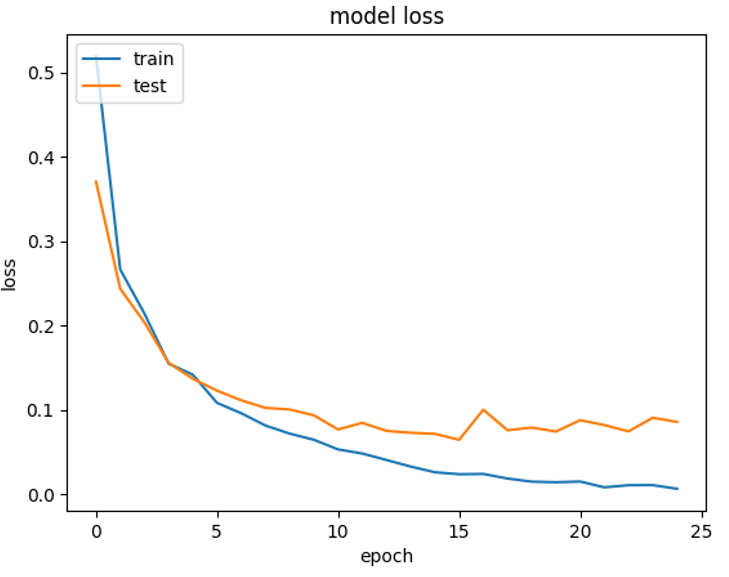
\includegraphics[width=0.5\textwidth]{lossmask.png} &
		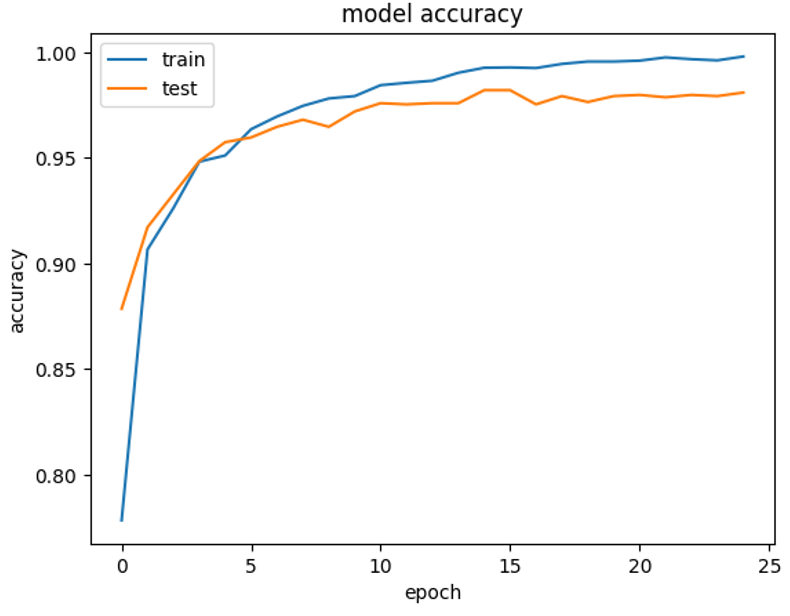
\includegraphics[width=0.5\textwidth]{accmask.png} 
	\end{tabular}
	\caption[Model Accuracy và Model Loss.]{Model Accuracy và Model Loss.}
	\label{fig:modelloss and Model Accuracy}
\end{figure}

Đồ thị ACC,  độ chính xác (Accuracy) lên đến 98\% và bắt đầu ổn định khi epoch = 10,  cho cả tập dữ liệu huấn luyện và tập test, đồ thị Loss của cũng cho thấy sau mức này, Loss của cả tập train và validation. Kết quả cho thấy mô hình có độ phù hợp tốt và không bị quá khớp (over-fitting).

\begin{itemize}
	\item Đánh giá hiệu suất mô hình:

	\begin{figure}[h!]
		\centering
		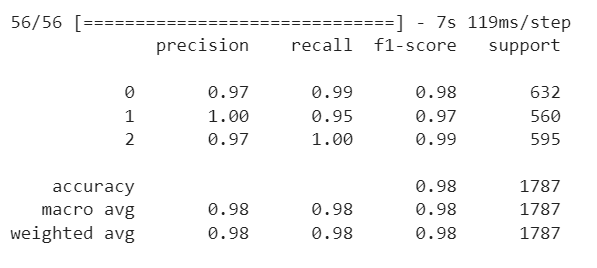
\includegraphics[width=0.6\textwidth]{per.png}
		\caption[Đánh giá hiệu suất mô hình.]{Đánh giá hiệu suất mô hình.}
		\label{fig:per} 
	\end{figure}

	\item Confusion Matrix:
		
	\begin{figure}[h!]
		\centering
		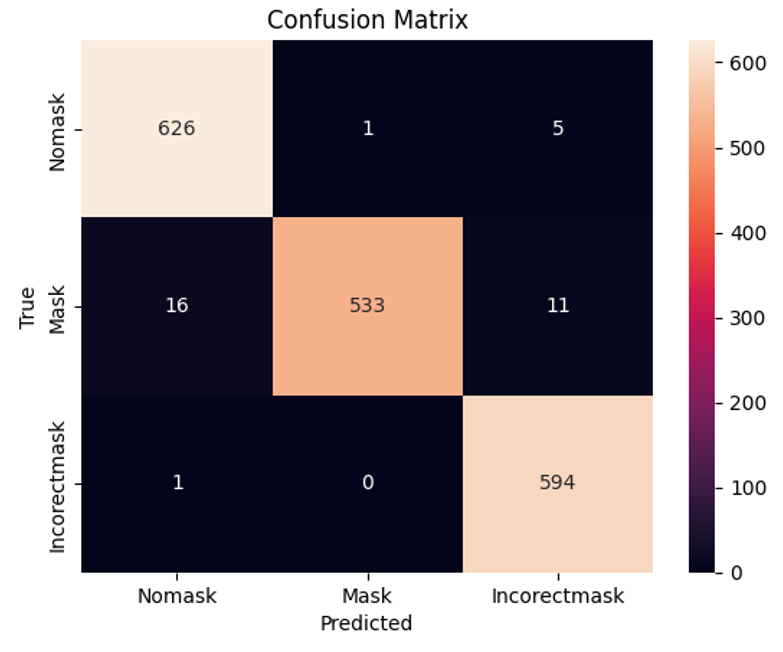
\includegraphics[width=0.53\textwidth]{confu.png}
		\caption[Confusion Matrix.]{Confusion Matrix.}
		\label{fig:confu} 
	\end{figure}
\end{itemize}

\subsubsection{Kết quả huất luyện tập dữ liệu cảm xúc}

\begin{figure}[h!] 
	\begin{tabular}{cc}
		\centering
		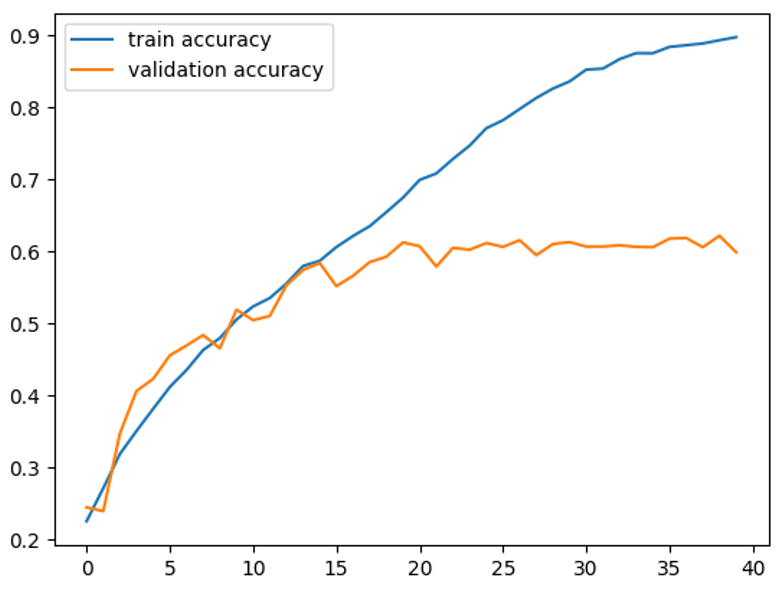
\includegraphics[width=0.5\textwidth]{accemotion.png} &
		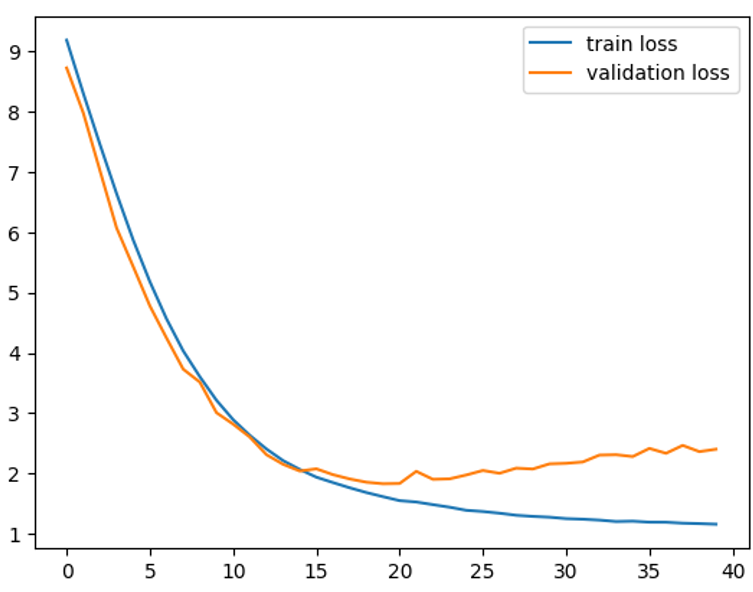
\includegraphics[width=0.5\textwidth]{lossemotion.png} 
	\end{tabular}
	\caption[Model Accuracy và Model Loss.]{Model Accuracy và Model Loss.}
	\label{fig:modelloss_and_Model Accuracy}
\end{figure}

Đồ thị ACC,  độ chính xác (Accuracy) lên đến 98\% ở tập train và 60\% ở tập test và bắt đầu ổn định khi epoch = 20,  cho cả tập dữ liệu huấn luyện và tập test, đồ thị Loss của cũng cho thấy sau mức này, Loss của cả tập train và validation. Kết quả cho thấy mô hình có độ phù hợp tốt và không bị quá khớp (over-fitting).

\begin{itemize}
	\item Đánh giá hiệu suất mô hình:
	
	\begin{figure}[h!]
		\centering
		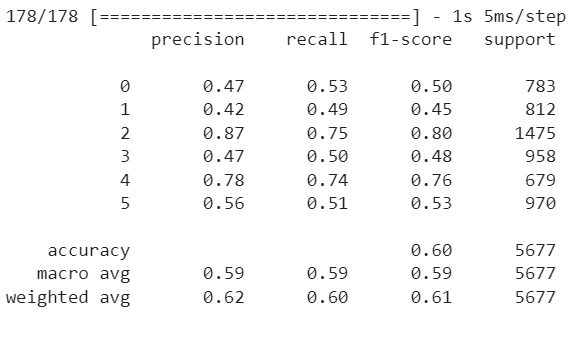
\includegraphics[width=0.7\textwidth]{ac.png}
		\caption[Đánh giá hiệu suất mô hình.]{Đánh giá hiệu suất mô hình.}
		\label{fig:ac} 
	\end{figure}
	
	\item Confusion Matrix:
	
	\begin{figure}[h!]
		\centering
		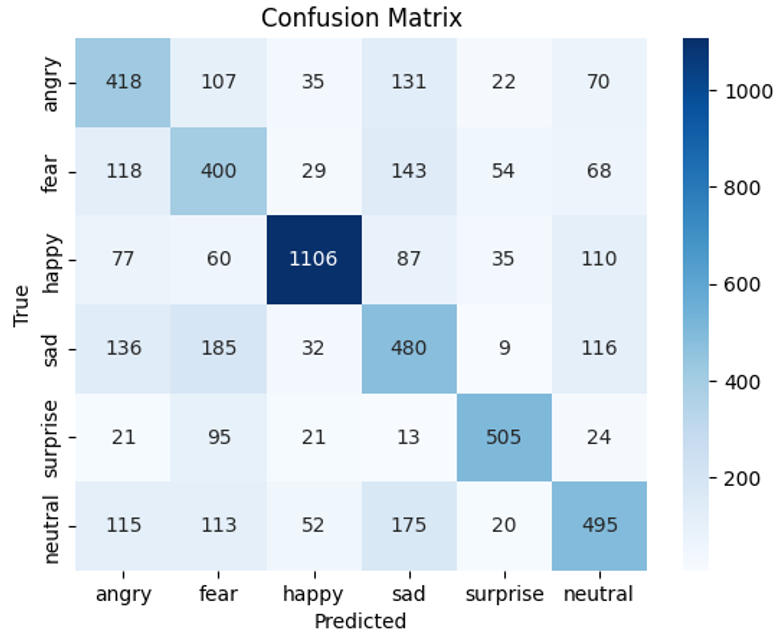
\includegraphics[width=0.6\textwidth]{fu.png}
		\caption[Confusion Matrix.]{Confusion Matrix.}
		\label{fig:fu} 
	\end{figure}
\end{itemize}

\subsection{Thử nghiệm với thời gian thực webcam}

*** Sử dụng thư viện open cv để test kết quả trên thời gian thực 

** Bước 1: Load Model

\begin{lstlisting}[style=codePython]
	from tensorflow.keras.models import load_model
	model1 = load_model('model_mask_final.h5')
	model2 = load_model('model_emotions_final.h5')					
\end{lstlisting}

** Bước 2: Phát hiện khuôn mặt

\begin{lstlisting}[style=codePython]
	prototxt = 'deploy.prototxt'
	model = 'res10_300x300_ssd_iter_140000.caffemodel'
	net = cv2.dnn.readNetFromCaffe(prototxt, model)						
\end{lstlisting}

** Bước 3: Chạy webcam

\begin{lstlisting}[style=codePython]
	cap = cv2.VideoCapture(0)
	
	while True:
	
	ret, frame = cap.read()
	
	if ret:       
		frame = imutils.resize(frame, width=500)
		(h, w) = frame.shape[:2]
		blob = cv2.dnn.blobFromImage(cv2.resize(frame, (300, 300)), 1.0, (300, 300), (104.0, 177.0, 123.0))
		net.setInput(blob)
		detections = net.forward()
		for i in range(0, detections.shape[2]):
			confidence = detections[0, 0, i, 2]
			if confidence > 0.5:
				box = detections[0, 0, i, 3:7] * np.array([w, h, w, h])
				(startX, startY, endX, endY) = box.astype("int")
				y = startY - 10 if startY - 10 > 10 else startY + 10
	
				minX, maxX = min(startX, endX), max(startX, endX)
				minY, maxY = min(startY, endY), max(startY, endY)
				face = frame[minY:maxY, minX:maxX].copy()
				img1 = cv2.resize(face,(48,48))
				img = np.array([img1/255.])
				y_ha = model1.predict(img)
				y_hat = np.argmax(y_ha)
				text= y_ha[0][y_hat]
				text = str(text)
				mask = ('Nomask', 'Mask', 'Incorect')
				predicted_mask = mask[y_hat] 
				cv2.rectangle(frame, (startX, startY), (endX, endY), (0, 0, 255), 2)
				cv2.putText(frame,predicted_mask, (startX, y),cv2.FONT_HERSHEY_SIMPLEX, 0.5, (255, 0, 0), 2) 
				cv2.putText(frame,text, (startX+70, y),cv2.FONT_HERSHEY_SIMPLEX, 0.5, (255, 0, 0), 2) 
				if y_hat ==0:                  
					img = cv2.cvtColor(img1,cv2.COLOR_BGR2GRAY)
					img = np.array([img/255.])
					y_ha2 = model2.predict(img)
					y_hat2 = np.argmax(y_ha2)
					k= y_ha2[0][y_hat2]
					text2 = str(k)
					emotions = ('angry', 'fear', 'happy', 'sad', 'surprise', 'neutral')
					predicted_emotion = emotions[y_hat2]
					cv2.putText(frame,predicted_emotion, (startX,endY+10),cv2.FONT_HERSHEY_SIMPLEX, 0.5, (0,255,0), 2)
					cv2.putText(frame,text2, (startX+70, endY+10),cv2.FONT_HERSHEY_SIMPLEX, 0.5, (255, 0, 0), 2)
	
		cv2.imshow("Detection", frame)
		key = cv2.waitKey(1)
		if key == 27:
			break
	cap.release()
	cv2.destroyAllWindows()							
\end{lstlisting}

**  Bước 4: Demo kết quả chạy webcam

\begin{figure}[h!]
	\centering
	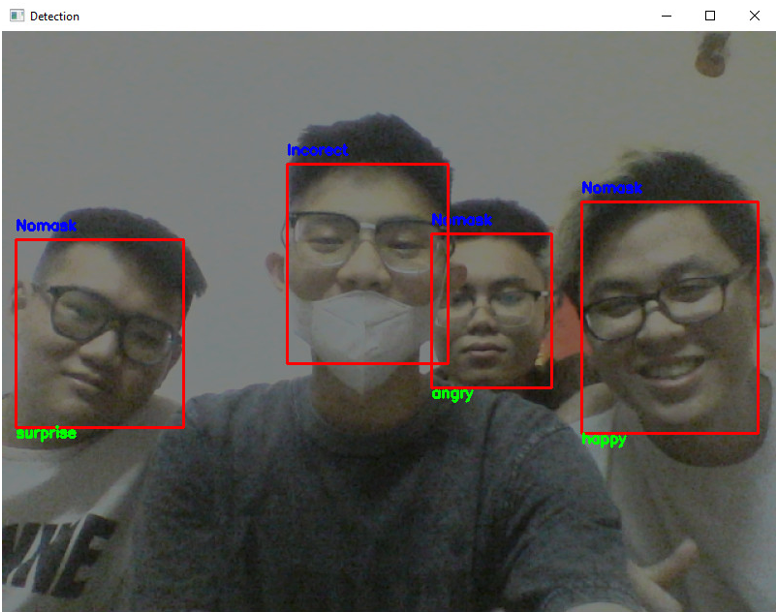
\includegraphics[width=0.6\textwidth]{demo1.png}
	\caption[Demo kết quả chạy webcam1.]{Demo kết quả chạy webcam1.}
	\label{fig:demo1} 
\end{figure}

\begin{figure}[h!]
	\centering
	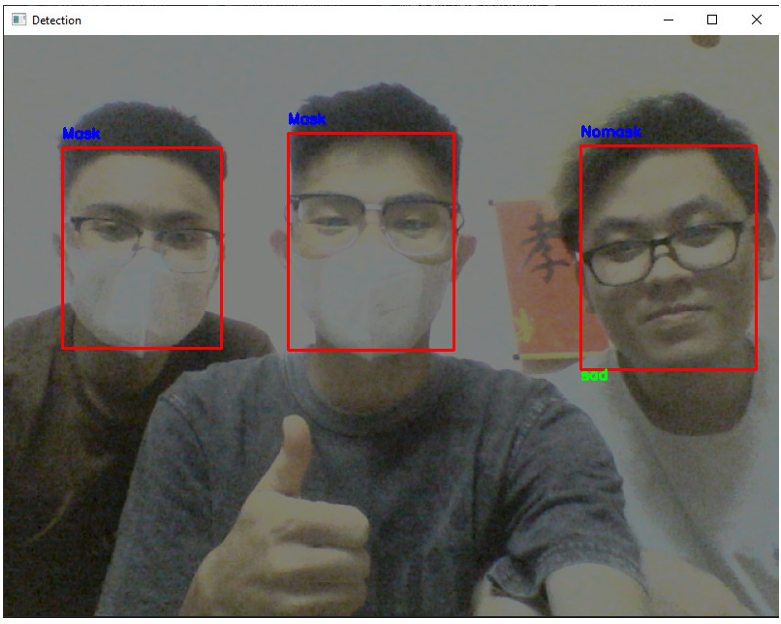
\includegraphics[width=0.7\textwidth]{demo2.png}
	\caption[Demo kết quả chạy webcam2.]{Demo kết quả chạy webcam2.}
	\label{fig:demo2} 
\end{figure}

\begin{figure}[h!] 
	\begin{tabular}{cc}
		\centering
		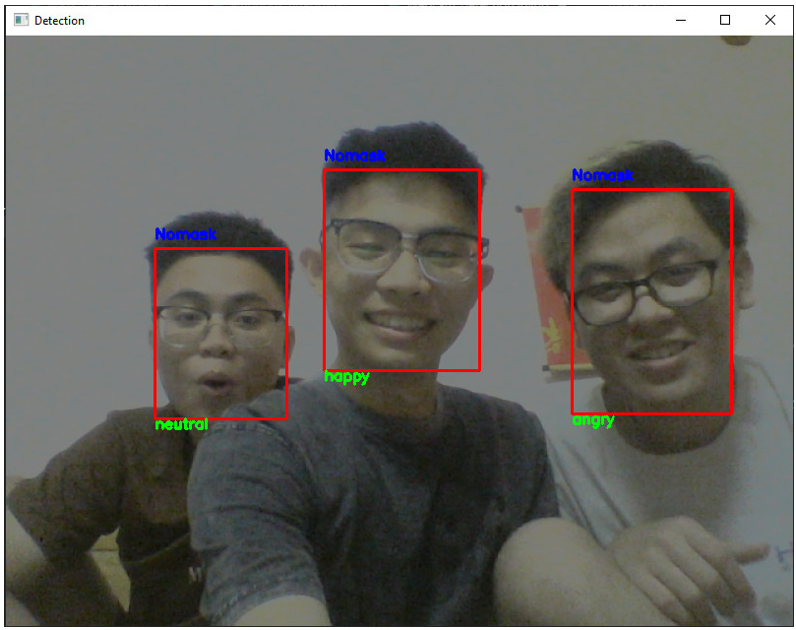
\includegraphics[width=0.5\textwidth]{demo3.png} &
		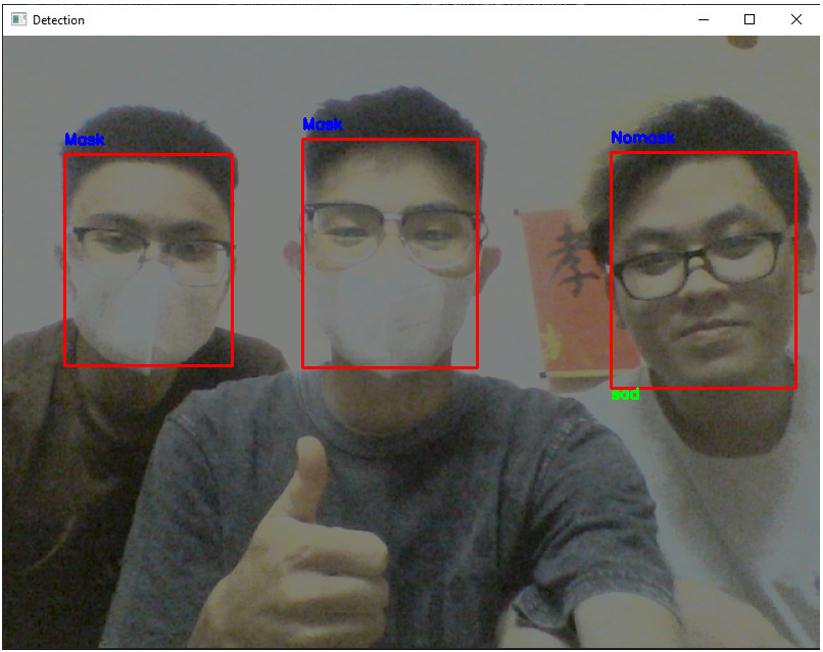
\includegraphics[width=0.5\textwidth]{demo4.png} 
	\end{tabular}
	\caption[Demo kết quả chạy webcam3.]{Demo kết quả chạy webcam3.}
	\label{fig:demo3}
\end{figure}









% Chương 4 

\chapter{KẾT QUẢ VÀ PHƯƠNG HƯỚNG PHÁT TRIỂN} 

\label{Chapter4}

\section{Kết quả}

Kết quả đạt được : Nhóm 2 đã ứng dụng thành công mạng neural tích chập trong việc phát hiện người có hay không đeo khẩu trang và nhận diện cảm xúc con người. Tuy nhiên dự án của nhóm vẫn còn một số những hạn chế nhất định, những ưu điểm và nhược điểm sau:

\subsection{Ưu điểm}

\begin{itemize}
	\item Tính ứng dụng: Tính ứng dụng cao, có thể linh hoạt sử dụng trong nhiều hoàn cảnh, địa điểm khác nhau. 
	
	\item Hiệu suất cao: CNN rất hiệu quả trong việc phân loại xác định hình ảnh, mô hình khẩu trang đã đạt được độ chính xác cao ( >98\%) trong việc phân loại người có hay không đeo khẩu trang.
	
	\item Xử lý được dữ liệu thời gian thực. 
\end{itemize}

\subsection{Nhược điểm}

\begin{itemize}
	\item Yêu cầu dữ liệu đủ lớn: Để đạt được hiệu suất tốt, mô hình CNN yêu cầu một lượng lớn dữ liệu. Điều này gây khó khăn trong việc phân loại cảm xúc khi mà lượng dữ liệu không được cân đối trong các lớp. 
	
	\item Tính chất dữ liệu có nhiều điểm chung: Khi thực hiện xác nhận có đeo khẩu trang, không đeo và đeo sai cách thì đeo sai cách rất khó phân biệt do có nhiều điểm giống với có đeo.
	
	\item Chưa được hoàn toàn chính xác và độ ổn định chưa được cao. 
\end{itemize}

\section{Hướng phát triển trong tương lai}

\begin{itemize}
	\item Trong tương lai, nhóm muốn tạo ra một app trên điện thoại để có thể đến được gần hơn với nhiều người. 
	
	\item Muốn phát triển lên thành sản phẩm hoàn chỉnh có tính thực tế cao hơn.	
	
	\item Không chỉ dừng lại ở việc xác định khẩu trang thêm vào đó là cảnh báo bằng âm thanh nếu thấy đối tượng không đeo khẩu trang. 
\end{itemize}



 
\chapter*{KẾT LUẬN}
\addcontentsline{toc}{chapter}{KẾT LUẬN}

\label{Chapter5}

Bài Báo cáo đã khái quát tầm quan trọng của chiếc khẩu trang đối với sức khỏe của con người trong thời kì dịch bệnh có nhiều diễn biến phức tạp, khó lường. Bên cạnh đó cũng đã ứng dụng Machine Learning (Học máy) vào việc nhận diện người dân có hay không đeo khẩu trang hoặc đeo sai cách và nhận diện được cảm xúc của họ theo thời gian thực.

Bài Báo cáo cung cấp khái niệm của mạng neural tích chập (Convolutional Neural Network - CNN), nắm được những thành phần cơ bản của một mô hình mạng neural, kiến trúc của mạng CNN, áp dụng được các thư viện (Numpy, OpenCV, Matplotlib, Tensorflow,...), để giải quyết vấn đề đã đặt ra từ trước. 

Đánh giá và khảo sát mô hình một cách nghiêm túc, thực tế, rút ra được những tiêu chí, yếu tố ảnh hưởng tới mô hình (Độ rõ ràng của tập dữ liệu, Chọn mô hình phù hợp, Quá trình huấn luyện,...), đánh giá mô hình (Độ chính xác, Hàm mất mất-Loss, Tính đồng nhất,...),...

Bài Báo cáo mới chỉ dừng lại ở mức độ nghiên cứu, bước đầu chạy thử nghiệm nhận biết khẩu trang và cảm xúc thành công, mô hình còn nhiều điểm chưa được ổn định, còn đơn giản, không quá phức tạp, đáp ứng một số tiêu chí nhất định để phù hợp với định hướng và mục tiêu mô học đề ra. Định hướng tương lai có thể thực hiện thành công và đưa vào phục vụ đời sống xã hội.









 



%----------------------------------------------------------------------------------------
%	(KHÔNG CHỈNH SỬA PHẦN NÀY)
%
%	PHẦN 10: TÀI LIỆU THAM KHẢO
%----------------------------------------------------------------------------------------

\begin{spacing}{1.15}
	\printbibliography[heading=bibintoc, title=Tài liệu tham khảo] % In ra tài liệu tham khảo
\end{spacing}

%\cite{Thiện_Thắng_Thặng_Bảo_2022,Reference2,Reference3,Reference4,Bisong2019}

%----------------------------------------------------------------------------------------
%	PHẦN 11: PHỤ LỤC (THESIS CONTENT - APPENDICES)
%----------------------------------------------------------------------------------------

%\appendix % Nói với LaTeX rằng những chương về sau được tính là phụ lục

% Hãy thêm những phụ lục (appendix) của khóa luận/tiểu luận vào thư mục Appendices
% Hãy bỏ chú thích những dòng nếu bạn đã bổ sung những phụ lục vào

\chapter*{Code}
\addcontentsline{toc}{chapter}{Code}

\label{Mã nguồn hệ thống}

***Một số code quan trọng trong hệ thống, các code còn lại đẩy trên google drive: \href{https://drive.google.com/drive/folders/1pspIib_DGpTEYfZ0l5Xm07Y1BCCl97d_?fbclid=IwAR1OaNPHzwGAtbG9NQQnDHE2cXxzpvXHW-w8ted6p9JCAnQck757pyKbOlw}{Source Code System} 

\section{Emotion Recognition}

\begin{lstlisting}
	import glob
	import shutil
	import cv2 
	from PIL import Image
	import PIL
	import os
	import numpy as np
	import pandas as pd
	import matplotlib.pyplot as plt
	import seaborn as sns
	import random 
	from sklearn.model_selection import train_test_split
	
	import warnings
	# Ignore waring
	warnings.filterwarnings('ignore')
	
	from google.colab import drive
	drive.mount('/content/drive')
	
	emotion_path = ['/angry/*', '/fear/*', '/happy/*', '/sad/*', '/surprise/*', '/neutral/*']
	Class_name = ['angry', 'fear', 'happy', 'sad', 'surprise', 'neutral']
	
	train_path = '/content/drive/MyDrive/Dataset/emotions/train'
	
	train_count=[]
	for i in Class_name:
	train_count.append(len(os.listdir("/content/drive/MyDrive/Dataset/emotions/train/"+i+"/")))
	plt.bar(Class_name,train_count)
	
	X = []
	y = []
	for i, path in enumerate(emotion_path):
	for name in glob.glob(train_path+path):
	img = cv2.imread(name)
	img = cv2.cvtColor(img,cv2.COLOR_BGR2GRAY)
	img = cv2.resize(img, (48,48))
	X.append((img))
	y.append(i)
	len(X)
	
	(X_train,X_test,y_train,y_test) = train_test_split(X,y,test_size=0.2,random_state=42)
	(X_train,X_val,y_train,y_val) = train_test_split(X_train,y_train,test_size=0.1,random_state=42)
	
	X_train = X_train /255
	X_val = X_val /255
	X_test = X_test / 255
	
	from sklearn.preprocessing import OneHotEncoder
	encoder = OneHotEncoder()
	encoder.fit(y_train.reshape(-1,1))
	y_train = encoder.transform(y_train.reshape(-1,1)).toarray()
	y_val = encoder.transform(y_val.reshape(-1,1)).toarray()
	y_test = encoder.transform(y_test.reshape(-1,1)).toarray()
	
	import numpy as np
	from matplotlib import pyplot as plt
	import tensorflow as tf
	import keras
	from keras.preprocessing import image
	from keras.models import Sequential
	from keras.layers import Conv2D, MaxPool2D, Flatten,Dense,Dropout,BatchNormalization
	from keras import regularizers
	
	import cv2
	model= tf.keras.models.Sequential()
	model.add(Conv2D(32, kernel_size=(3, 3), padding='same', activation='relu', input_shape=(48, 48,1)))
	model.add(Conv2D(64,(3,3), padding='same', activation='relu' ))
	model.add(BatchNormalization())
	model.add(MaxPool2D(pool_size=(2, 2)))
	model.add(Dropout(0.25))
	
	model.add(Conv2D(128,(5,5), padding='same', activation='relu'))
	model.add(BatchNormalization())
	model.add(MaxPool2D(pool_size=(2, 2)))
	model.add(Dropout(0.25))
	
	model.add(Conv2D(512,(3,3), padding='same', activation='relu', kernel_regularizer=regularizers.l2(0.01)))
	model.add(BatchNormalization())
	model.add(MaxPool2D(pool_size=(2, 2)))
	model.add(Dropout(0.25))
	
	model.add(Conv2D(512,(3,3), padding='same', activation='relu', kernel_regularizer=regularizers.l2(0.01)))
	model.add(BatchNormalization())
	model.add(MaxPool2D(pool_size=(2, 2)))
	model.add(Dropout(0.25))
	
	model.add(Flatten()) 
	model.add(Dense(256,activation = 'relu'))
	model.add(BatchNormalization())
	model.add(Dropout(0.25))
	
	model.add(Dense(512,activation = 'relu'))
	model.add(BatchNormalization())
	model.add(Dropout(0.25))
	
	model.add(Dense(6, activation='softmax'))
	
	from keras.utils.vis_utils import plot_model 
	plot_model(model,show_shapes=True,show_layer_names=True)
	
	learning_rate = 0.0001  # Toc do hoc ban dau
	
	# Khoi tao learning rate scheduler
	optimizer1 = tf.keras.optimizers.Adam(learning_rate = 0.0001)
	
	model.compile(optimizer = optimizer1, loss = 'categorical_crossentropy',metrics =['accuracy'])
	
	history = model.fit(X_train, y_train,
	epochs=40,validation_data=(X_val, y_val),batch_size = 64,shuffle = True)
	
	h = history
	
	# plot the loss value
	plt.plot(h.history['loss'], label='train loss')
	plt.plot(h.history['val_loss'], label='validation loss')
	plt.legend()
	plt.show()
	
	#plot the accuracy value
	plt.plot(h.history['accuracy'], label='train accuracy')
	plt.plot(h.history['val_accuracy'], label='validation accuracy')
	plt.legend()
	plt.show()
	
	model.save('model_emotions_final_67.h5')
	
	from sklearn.metrics import confusion_matrix, classification_report, accuracy_score
	y_hat = model1.predict(X_test)
	y_test1 =np.argmax(y_test,axis =1)
	y_hat1 = np.argmax(y_hat,axis =1)
	print(classification_report(y_test1, y_hat1))
	
	import seaborn as sns
	
	cm = confusion_matrix(y_test1, y_hat1)
	print(cm)
	sns.heatmap(cm, annot=True, fmt='d', cmap='Blues')
	
	# Cau hinh truc x va truc y 
	tick_labels = ['angry', 'fear', 'happy', 'sad', 'surprise', 'neutral']
	plt.xticks(np.arange(len(tick_labels)) + 0.5, tick_labels)
	plt.yticks(np.arange(len(tick_labels)) + 0.5, tick_labels)
	
	#Dat ten cac truc 
	plt.xlabel('Predicted')
	plt.ylabel('True')
	
	# Hien thi bieu do
	plt.title('Confusion Matrix')
	plt.show()
\end{lstlisting}

\section{Mask Detection}

\begin{lstlisting}
	import matplotlib.image as mpimg
	import glob
	import shutil
	import cv2 
	from PIL import Image
	import PIL
	import os
	import numpy as np
	import pandas as pd
	import matplotlib.pyplot as plt
	from sklearn.metrics import confusion_matrix
	import seaborn as sns
	from sklearn.model_selection import train_test_split
	import tensorflow
	from tensorflow.keras.models import Model
	from tensorflow.keras.layers import Dense, Dropout, Flatten, Input, Reshape
	from tensorflow.keras.layers import Conv2D, MaxPooling2D
	
	import warnings
	# Ignore waring
	warnings.filterwarnings('ignore')
	
	Class_name = ['without_mask', 'with_mask', 'mask_weared_incorrect']
	train_count=[]
	for i in Class_name:
	train_count.append(len(os.listdir("dataset/"+i+"/")))
	plt.bar(Class_name,train_count)
	
	mask_path = ['/without_mask/*','/with_mask/*','/mask_weared_incorrect/*' ]
	train_path = 'dataset'
	
	X = []
	y = []
	for i, path in enumerate(mask_path):
	for name in glob.glob(train_path + path):
	img = cv2.imread(name)
	img = cv2.cvtColor(img,cv2.COLOR_BGR2RGB)
	img = cv2.resize(img,(48,48))
	X.append((img))
	y.append(i)
	len(X)
	
	# np.array
	X = np.array(X)/255.
	y = np.array(y)
	
	X_train, X_test, y_train, y_test = train_test_split(X,y, test_size=0.2, random_state=2)
	
	from sklearn.preprocessing import OneHotEncoder
	encoder = OneHotEncoder()
	encoder.fit(y_train.reshape(-1,1))
	y_train = encoder.transform(y_train.reshape(-1,1)).toarray()
	y_test = encoder.transform(y_test.reshape(-1,1)).toarray()
	print(y_train)
	
	#CNN
	inp = Input(shape = (48,48,3))
	cnn = Conv2D(filters =16,kernel_size = 3,activation ='relu')(inp)
	pooling = MaxPooling2D(pool_size =(2,2))(cnn)
	drop = Dropout(0.2)(pooling)
	
	cnn = Conv2D(filters =32,kernel_size = 3,activation ='relu')(inp)
	pooling = MaxPooling2D(pool_size =(2,2))(cnn)
	drop = Dropout(0.2)(pooling)
	
	cnn = Conv2D(filters =64,kernel_size = 4,activation ='relu')(inp)
	pooling = MaxPooling2D(pool_size =(2,2))(cnn)
	drop = Dropout(0.2)(pooling)
	
	cnn = Conv2D(filters =128, kernel_size =4,activation ='relu')(drop)
	pooling = MaxPooling2D(pool_size =(2,2))(cnn)
	drop = Dropout(0.2)(pooling)
	
	f =Flatten()(pooling)
	
	fc1 = Dense(units =128, activation ='relu')(f)
	fc2 = Dense(units =64, activation ='relu')(fc1)
	fc3 = Dense(units =32, activation ='relu')(fc2)
	out = Dense(units =3, activation ='softmax')(fc3)
	
	model =Model(inputs = inp,outputs =out)
	model.summary()
	
	optimizer1 = tensorflow.keras.optimizers.Adam(learning_rate = 0.0001)
	model.compile(optimizer = optimizer1, loss = 'categorical_crossentropy',metrics =['accuracy'])
	
	history = model.fit(X_train,y_train,batch_size =16, epochs =25,validation_data =(X_test,y_test))
	
	from matplotlib import pyplot  as plt
	plt.plot(history.history['accuracy'])
	plt.plot(history.history['val_accuracy'])
	plt.title('model accuracy')
	plt.ylabel('accuracy')
	plt.xlabel('epoch')
	plt.legend(['train','test'],loc ='upper left')
	plt.show()
	#summarize history for loss
	plt.plot(history.history['loss'])
	plt.plot(history.history['val_loss'])
	plt.title('model loss')
	plt.ylabel('loss')
	plt.xlabel('epoch')
	plt.legend(['train','test'],loc ='upper left')
	plt.show()
	
	model.save('model2.h5')
	
	from sklearn.metrics import classification_report
	y_hat = model1.predict(X_test)
	y_test1 =np.argmax(y_test,axis =1)
	y_hat1 = np.argmax(y_hat,axis =1)
	print(classification_report(y_test1, y_hat1))
	
	matrix = confusion_matrix(y_test1,y_hat1)
	print(matrix)
	sns.heatmap(matrix, annot=True, fmt='d')
	
	tick_labels = ['Nomask', 'Mask','Incorectmask']
	plt.xticks(np.arange(len(tick_labels)) + 0.5, tick_labels)
	plt.yticks(np.arange(len(tick_labels)) + 0.5, tick_labels)
	
	#Dat ten cho cac truc
	plt.xlabel('Predicted')
	plt.ylabel('True')
	
	#Hien thi bieu do
	plt.title('Confusion Matrix')
	plt.show()
\end{lstlisting}


%\include{Appendices/AppendixB}
%\include{Appendices/AppendixC}

%----------------------------------------------------------------------------------------

\end{document}  
